\appendix

%\section*{\begin{center}{\Huge Appendix A: bleh}\end{center}}
%\addcontentsline{toc}{chapter}{Appendix A}
\chapter{Complimentary Results}
\label{sec:AppendixA}

\section{Determining sample parameters}
\label{appendix:sample_parameters}
\text{\color{red}flytt til Resultatdel "effect of mound"??}
\begin{itemize}
    \item First assumed to have mound around 20 nm, as the initial deposited film thickness of gold was 20nm for sample 6 and the total height of mound+particle was found to be around 40nm.
    \item When increasing the height of particle in the case of no mound present, the LSPR was found to resonate at lower wavelength and the reflectance smaller. Figure \ref{fig:S6_Rz_sweep_nomound}.
    \item Introducing the mound greatly dampened (almost halved) the reflectance. It also moved the LSPR to lower wavelength (e.g. Rz=20nm no mound has LSPR@635nm, with 19nm mound LSPR@610nm). Figure \ref{fig:S6_Rz_sweep_mound_1}
    \item Experimental LSPR peak was found to be at around 577nm for $\phi_0=0^\circ$. (varying between 567-582nm for the whole 0-360 rotation)
    \item The mound height was therefore further reduced until matched better with experimental LSPR location.
    \item The parameters [Rz=32, t=8] through [Rz=35,t=5] all had LSPR peak centered at 580 nm (a smaller wavelength stepsize would be needed to resolve these), although the resonance strength varied slightly.
    \item A mound height of $t=8$nm was chosen. A smaller mound height is more difficult geometry to handle from a meshing point of view, as it would create in sharp mesh edges/tips resulting in tiny elements. Having tiny elements compared to the rest of the geometry basically means having more elements to solve than strictly necessary. These sharp tipped elements along the edges of the mound also results in lower mesh quality, though this is only expected to have a slight effect on the accuracy of the results locally. In the big picture it may not be important.
\end{itemize}

\text{\color{red}re-plot in matlab for readability}
\begin{figure}[h!]
    \centering
    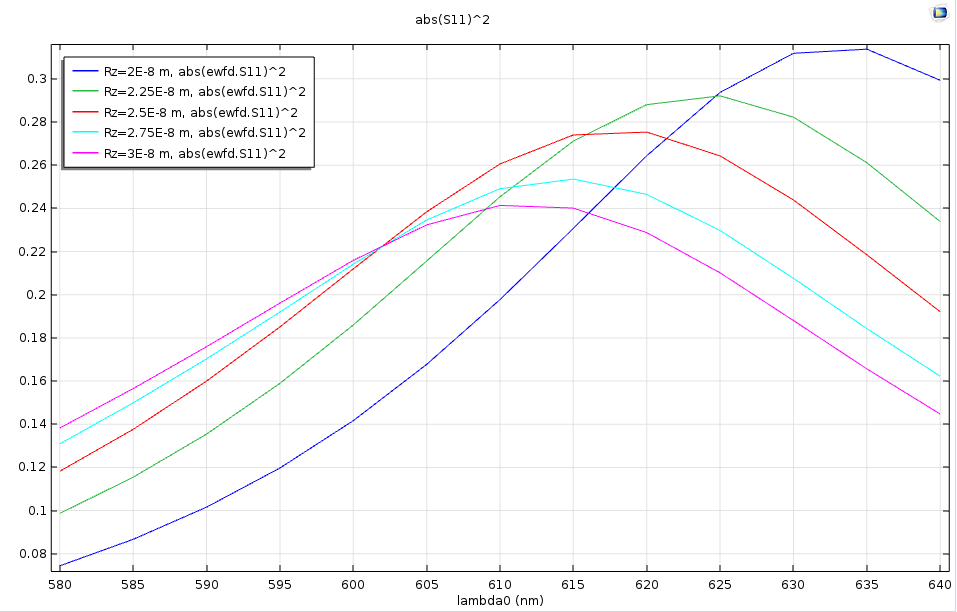
\includegraphics[width=0.6\linewidth]{figures/Appendix/parameters/Sample6_TM_NoMound_phi0_theta0_wl580-640_Rz20-30_absS11squared.png}
    \caption{no mound}
    \label{fig:S6_Rz_sweep_nomound}
\end{figure}
\begin{figure}[h!]
    \centering
    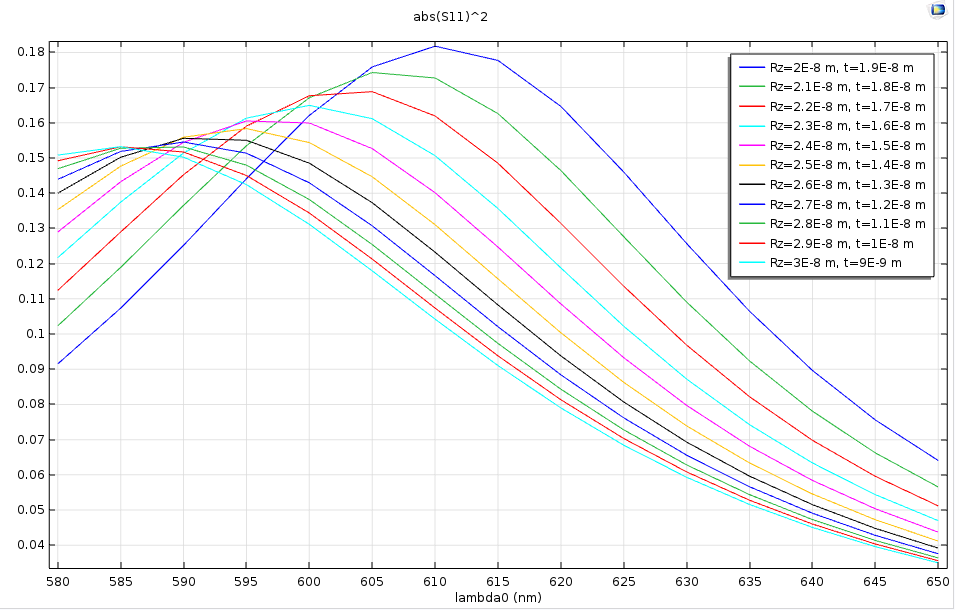
\includegraphics[width=0.6\linewidth]{figures/Appendix/parameters/Sample6_TM_Mound_phi0_theta55_wl580-650_Rz20-30_t9-19_absS11squared.png}
    \caption{mound}
    \label{fig:S6_Rz_sweep_mound_1}
\end{figure}
\begin{figure}[h!]
    \centering
    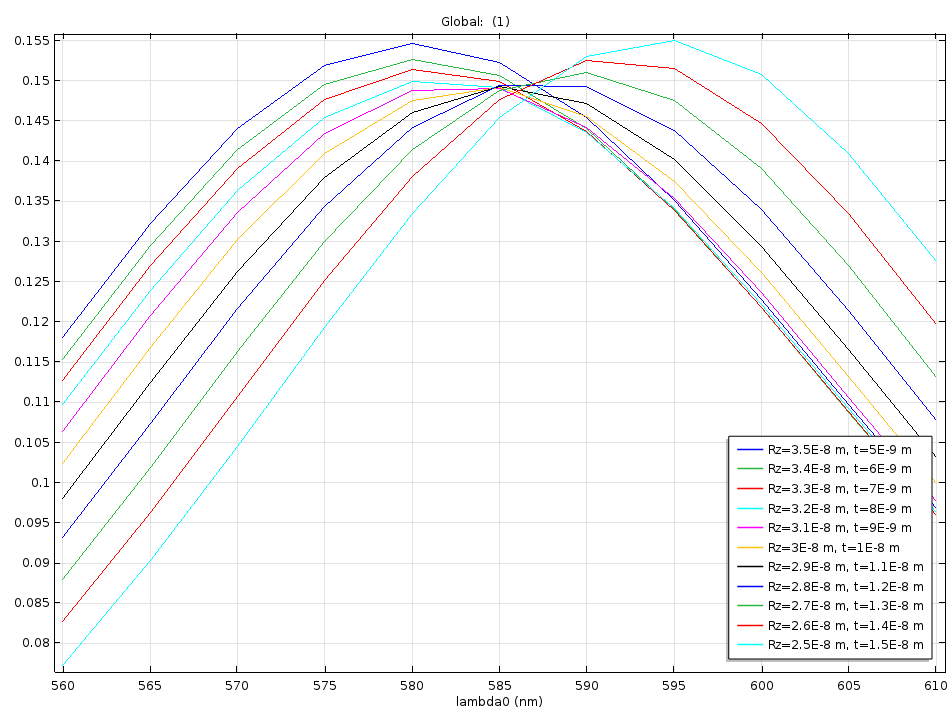
\includegraphics[width=0.6\linewidth]{figures/Appendix/parameters/Sample6_TM_Mound_phi0_theta55_wl560-610_Rz25-35_t5-15_absS11squared.png}
    \caption{Sample 6. Different sets of sample parameters $R_z$ and $t$ swept over the wavelength region expected to find a LSPR.}
\end{figure}


\begin{figure}[h!]
    \centering
    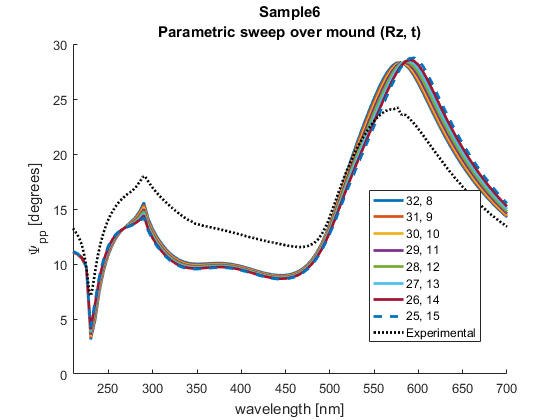
\includegraphics[width=0.8\linewidth]{figures/Appendix/parameters/Sample6_Psipp_varying_Rz_and_t_mound_parameters.png}
\end{figure}

\begin{itemize}
    \item Kort om å bruke GranFilm til å reversere eksperimentaldata til å finne sample parametre?
\end{itemize}

\section{Improvements upon Model}
lkdjbgdgh  fghf hfdh fhfg hfh fgh fgh fgh
gfhf ghd fhf gh fgh fgh 
\begin{figure}
    \centering
    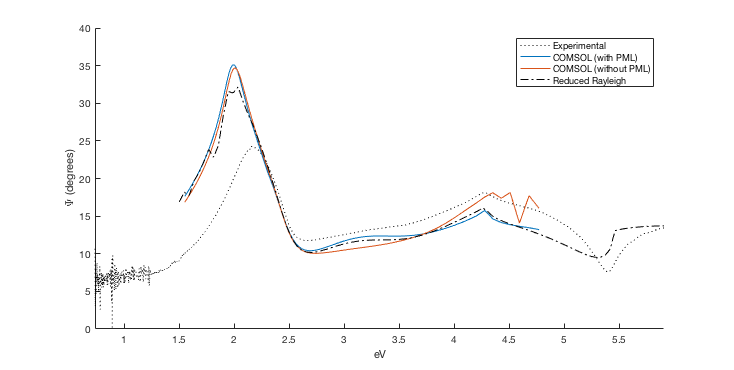
\includegraphics[scale=0.5]{figures/Appendix/Psi_ComsolPMLvsJPvsUserports.png}
    \caption{Early version of the COMSOL model comparing before and after implementation of PMLs.}
    \label{fig:Appendix_PMLvsnoPML}
\end{figure}
khgfkhfkckck lkdjbgdgh  fghf hfdh fhfg hfh fgh fgh fgh
gfhf ghd fhf gh fgh fgh 

%\begin{figure}
%    \centering
%    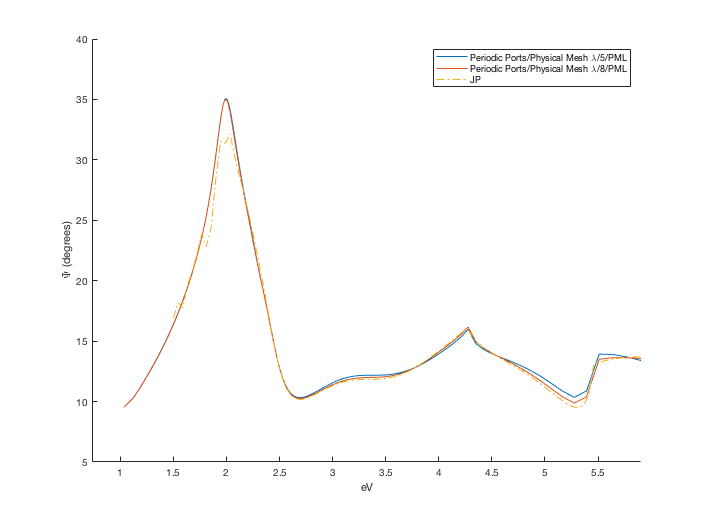
\includegraphics[scale=0.4]{figures/Appendix/Psi_ComsolPMLvsJP_2_.png}
%    \caption{S6}
%    \label{fig:Appendix_Convergence}
%    \change{change figure. finn data og plot ny, evt kjør ny sim og sammenlikn}
%\end{figure}

\begin{figure}
    %\centering
    \begin{subfigure}{.5\textwidth}
        \centering %width=.8\linewidth
        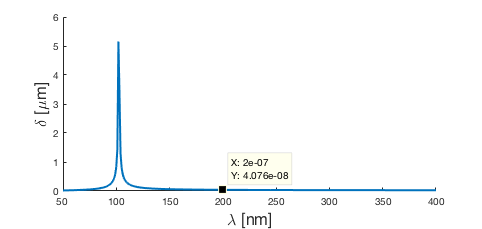
\includegraphics[width=\linewidth,trim=0.5cm 0cm 1cm 0cm, clip]{figures/Appendix/DecayLengthOfDiffractedMode_Sample6.png}
        \caption{Sample 6}
        \label{}
    \end{subfigure}
    \begin{subfigure}{.5\textwidth}
        \centering %width=.8\linewidth
        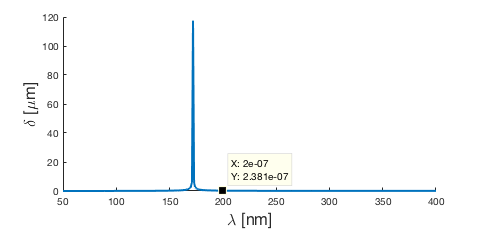
\includegraphics[width=\linewidth,trim=0.5cm 0cm 1cm 0cm, clip]{figures/Appendix/DecayLengthOfDiffractedMode_Sample5A.png}
        \caption{Sample 5A}
        \label{}
    \end{subfigure}
    \\
    \begin{subfigure}{.5\textwidth}
        \centering %width=.8\linewidth
        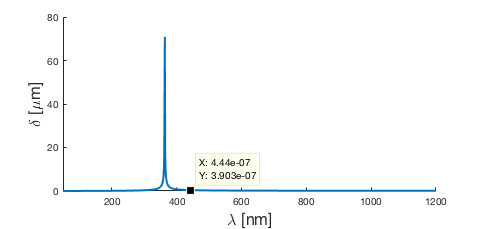
\includegraphics[width=\linewidth,trim=0.5cm 0cm 1cm 0cm, clip]{figures/Appendix/DecayLengthOfDiffractedMode_Sample5B.png}
        \caption{Sample 5B}
        \label{}
    \end{subfigure}
    \begin{subfigure}{.5\textwidth}
        \centering
        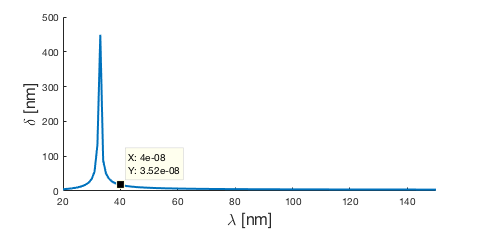
\includegraphics[width=\linewidth,trim=0.5cm 0cm 1cm 0cm, clip]{figures/Appendix/DecayLengthOfDiffractedMode_GaSbCones_assumingsquarelattice1.png}
        \caption{Tilted GaSb Cones}
        \label{fig:}
    \end{subfigure}
    \caption{Placeholder text. Decay length $\delta=\text{Im}[k_{z1}]^{-1}$ of first cut-off diffraction mode $k_{z1}=\sqrt{k^2-(2\pi/a-k_x)^2}$. Datapoints marked show the smallest wavelength each sample is simulated for \color{red}FIX: 5A(210nm) 5B(250nm) GaSb(??). I følge plot vil diffraksjonsmoder nå fram til PML, men resultatene virker ikke påvirket (3.2-3.4eV)??}
    \label{fig:Appendix_DecayLength}
\end{figure}
Figure \ref{fig:Appendix_DecayLength} tells us the minimum required distance from point of reflection to PML, as the PMLs supposedly(?) do not absorb evanescent diffraction modes. It is desirable, for practical reasons, to have as short a spacing between these points as possible without it affecting results. This can greatly reduce computation time and memory usage. Each sample is simulated with this distance being equal to its nearest particle neighbour. 

\subsubsection*{Minimizing the problem size \color{red}flytt der det passer}
\begin{itemize}
    \item Simplify the problem: solve in 2D instead of 3D (e.g. if the dependency along one direction is known. The solution may even be more accurate as a much denser mesh can be used), find symmetries in the geometry
    \item Use efficient boundary conditions, truncating the geometry without introducing too large errors: PMLs where the model geometry extends to infinity, replace thin layers with BCs
    \item Meshing: try to remove details that do not influence the solution as they produce alot of unnecessary mesh elements. The mesh generator automatically generates a finer mesh where there is a lot of fine geometrical details. Resolve the wavelength; about 10 linear (or 5 2nd order) elements per wavelength, and dependent on material.
    
\end{itemize}

\section{Sample 6}


\section{Sample 5A}
\begin{figure}[htb!]  %% FIELD DISTRIBUTION 210-500 nm
    \begin{subfigure}{0.32\textwidth}    %% TE
        \centering
        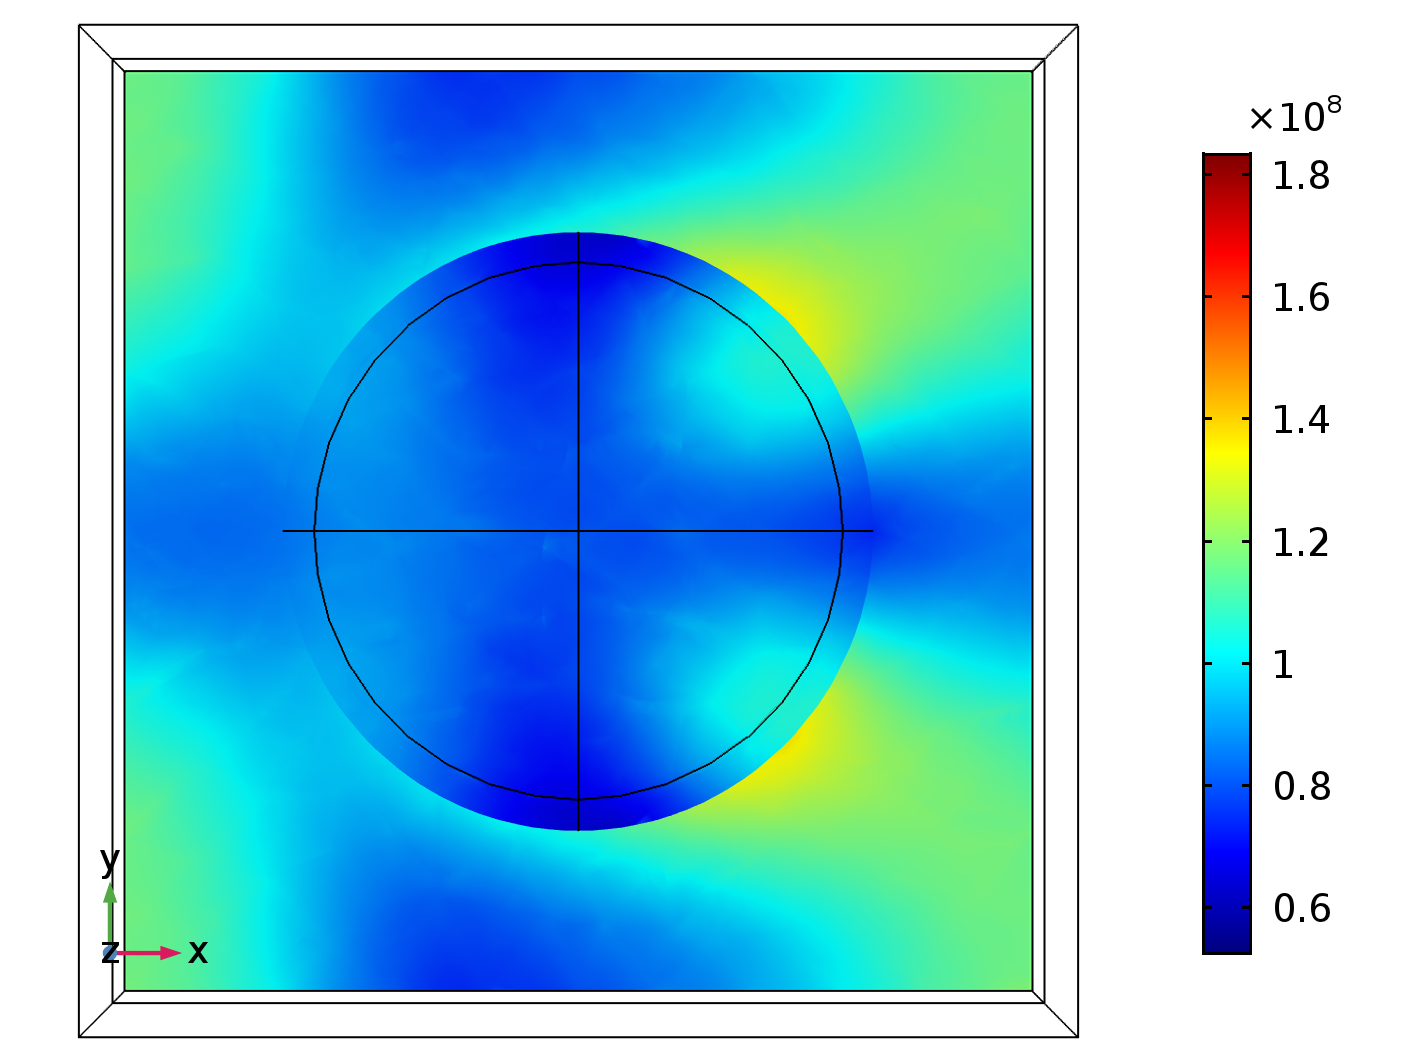
\includegraphics[width=\linewidth]{figures/ch4/S5A/FieldDistribution/Sample5A_TE_Slice@z=-05t_wl=210_notitle.png}
        %\caption{}
   \end{subfigure}
   \begin{subfigure}{0.32\textwidth}
        \centering
        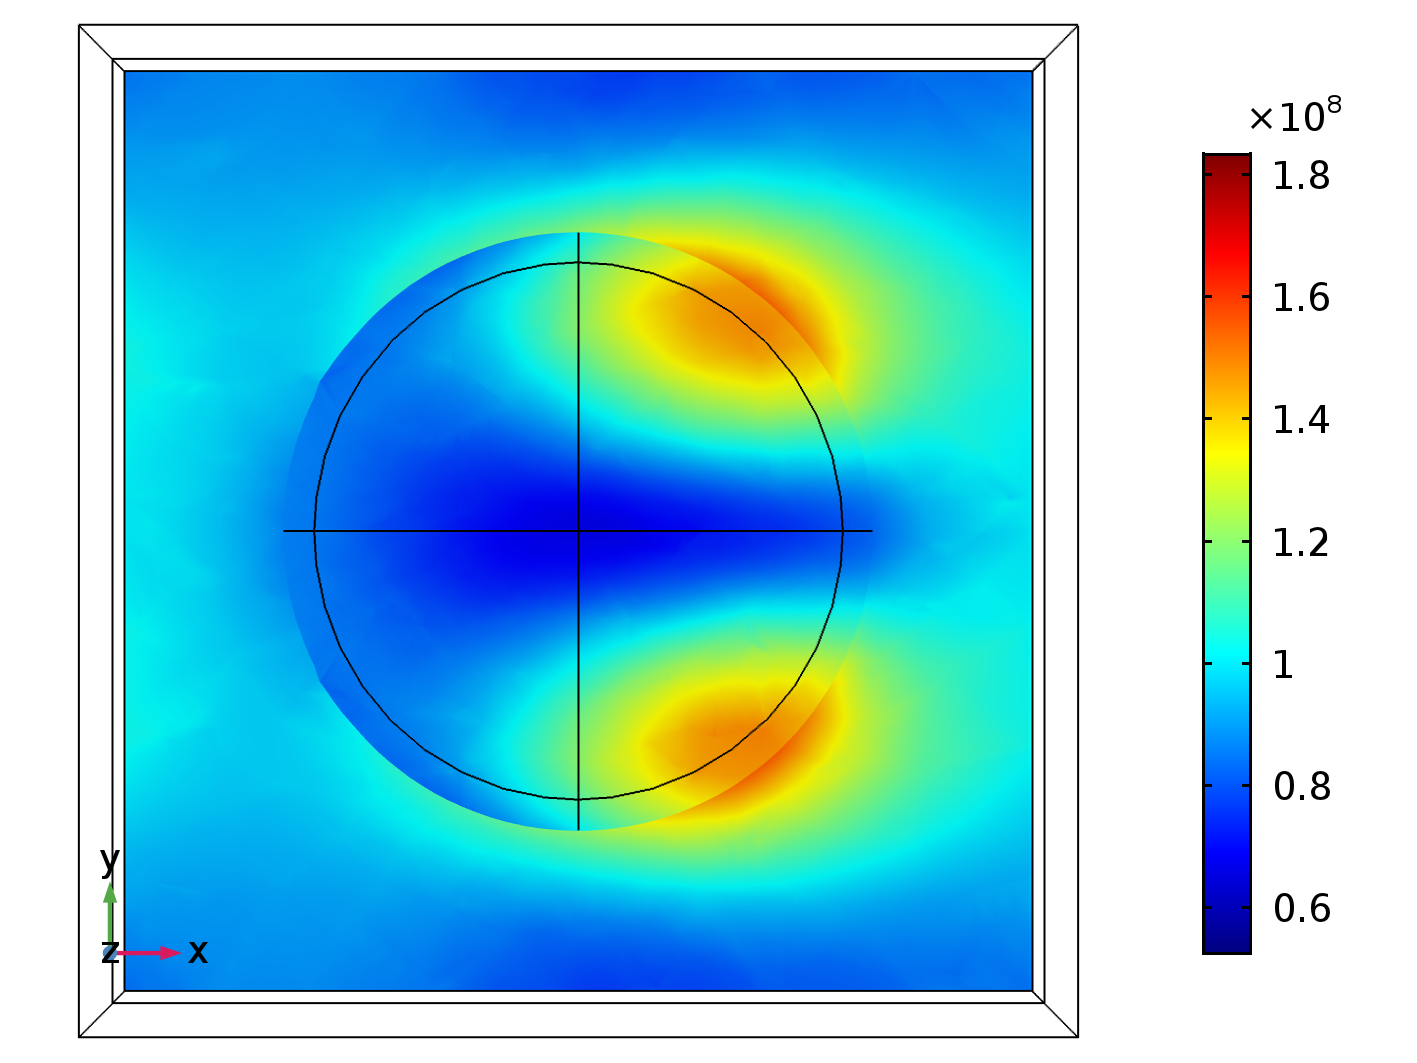
\includegraphics[width=\linewidth]{figures/ch4/S5A/FieldDistribution/Sample5A_TE_Slice@z=-05t_wl=270_notitle.png}
        %\caption{}
   \end{subfigure}
   \begin{subfigure}{0.32\textwidth}
        \centering
        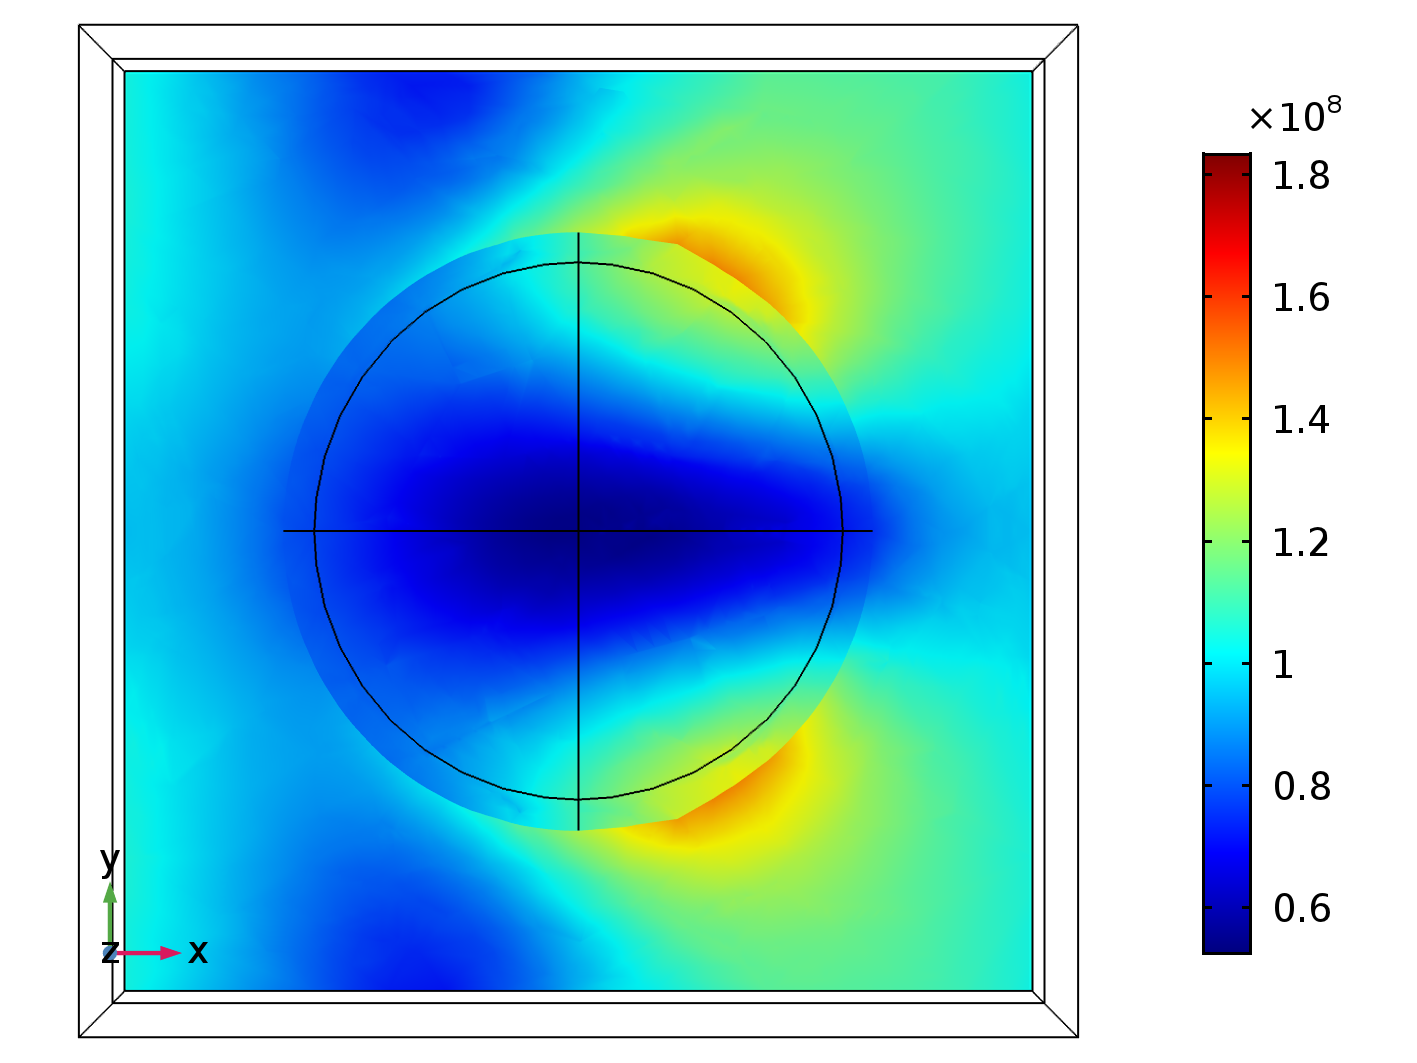
\includegraphics[width=\linewidth]{figures/ch4/S5A/FieldDistribution/Sample5A_TE_Slice@z=-05t_wl=330_notitle.png}
        %\caption{}
   \end{subfigure}

    \begin{subfigure}{0.32\textwidth}
        \centering
        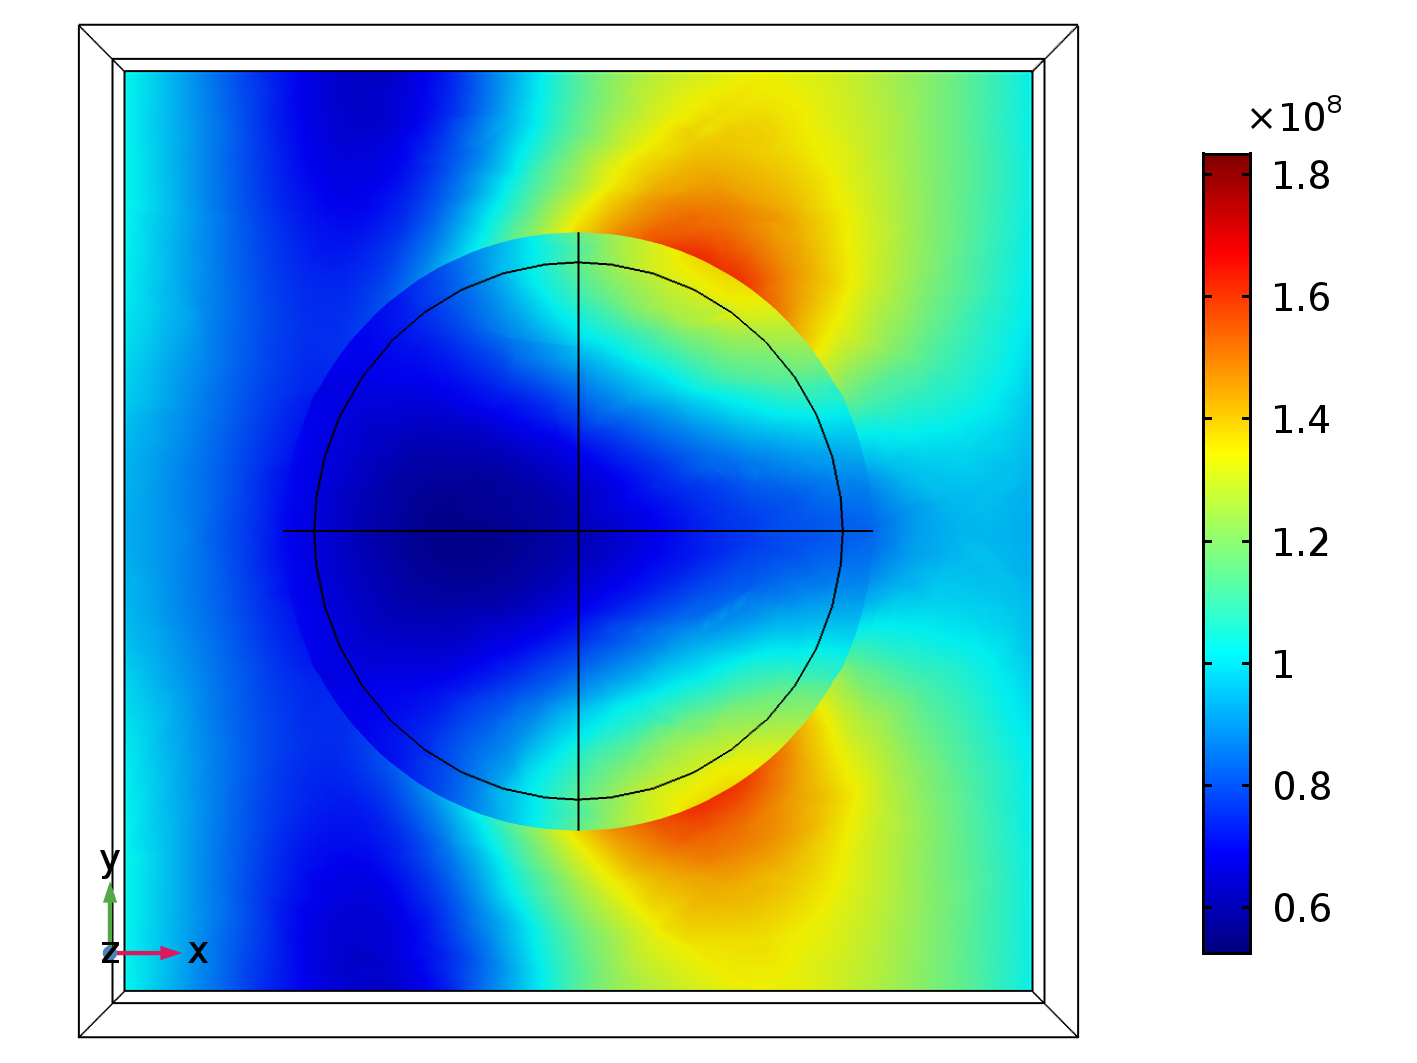
\includegraphics[width=\linewidth]{figures/ch4/S5A/FieldDistribution/Sample5A_TE_Slice@z=-05t_wl=390_notitle.png}
        %\caption{}
   \end{subfigure}
   \begin{subfigure}{0.32\textwidth}
        \centering
        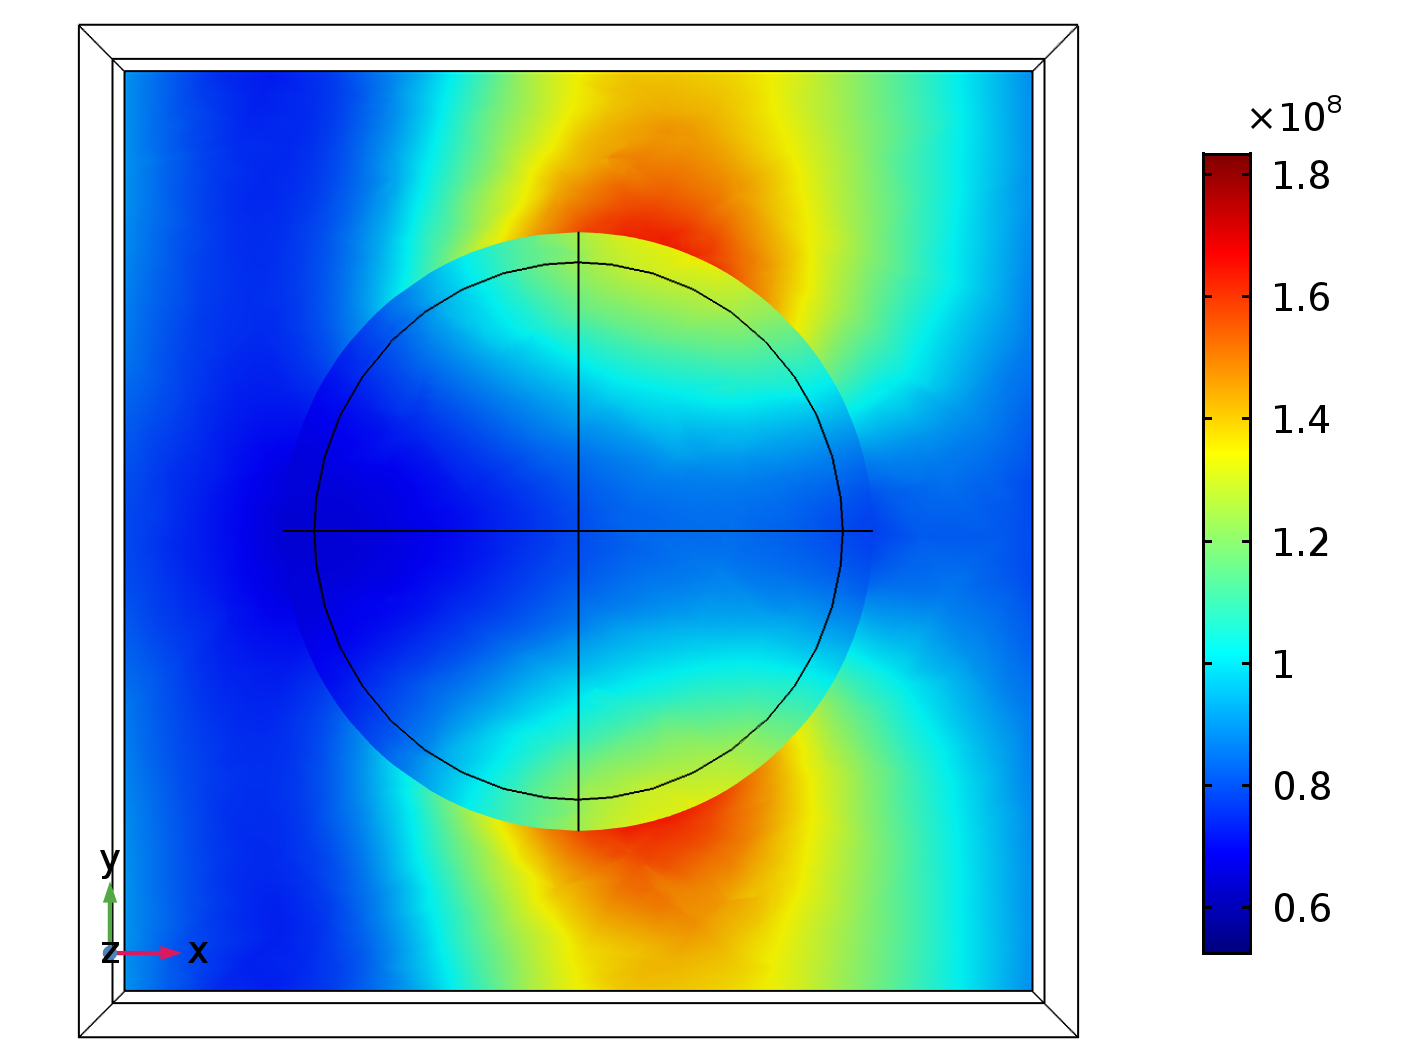
\includegraphics[width=\linewidth]{figures/ch4/S5A/FieldDistribution/Sample5A_TE_Slice@z=-05t_wl=450_notitle.png}
        \caption{TE}
        \vspace{-0.7cm}
   \end{subfigure}
   \begin{subfigure}{0.32\textwidth}
        \centering
        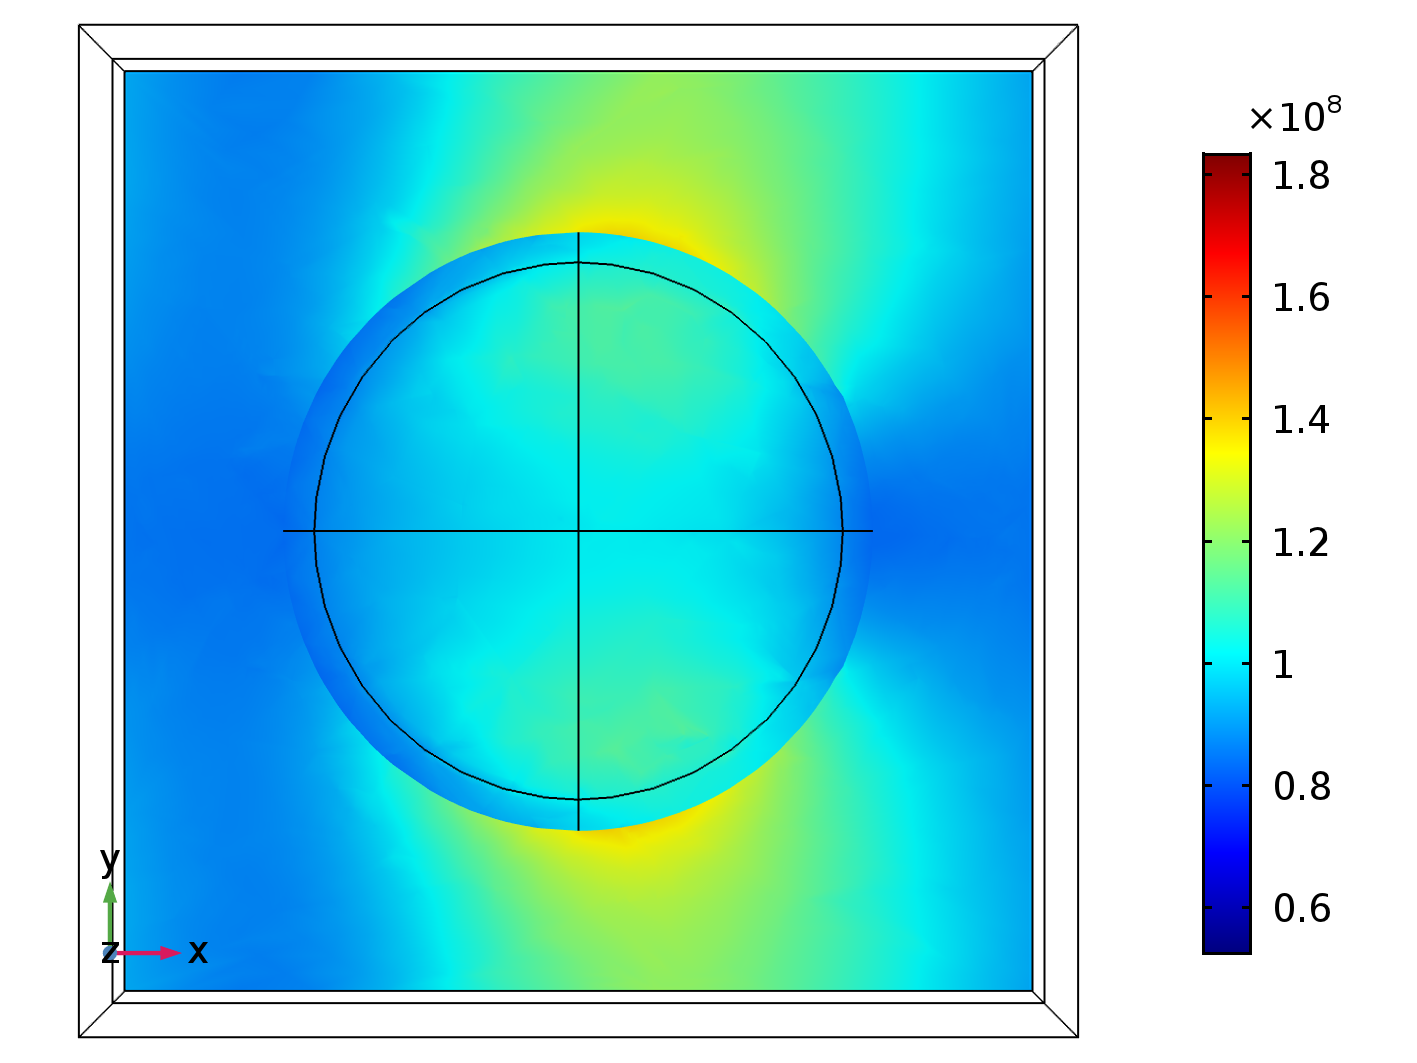
\includegraphics[width=\linewidth]{figures/ch4/S5A/FieldDistribution/Sample5A_TE_Slice@z=-05t_wl=500_notitle.png}
        %\caption{}
   \end{subfigure}
   \vspace{0.7cm}
   
   \begin{subfigure}{0.32\textwidth}    %% TM
        \centering
        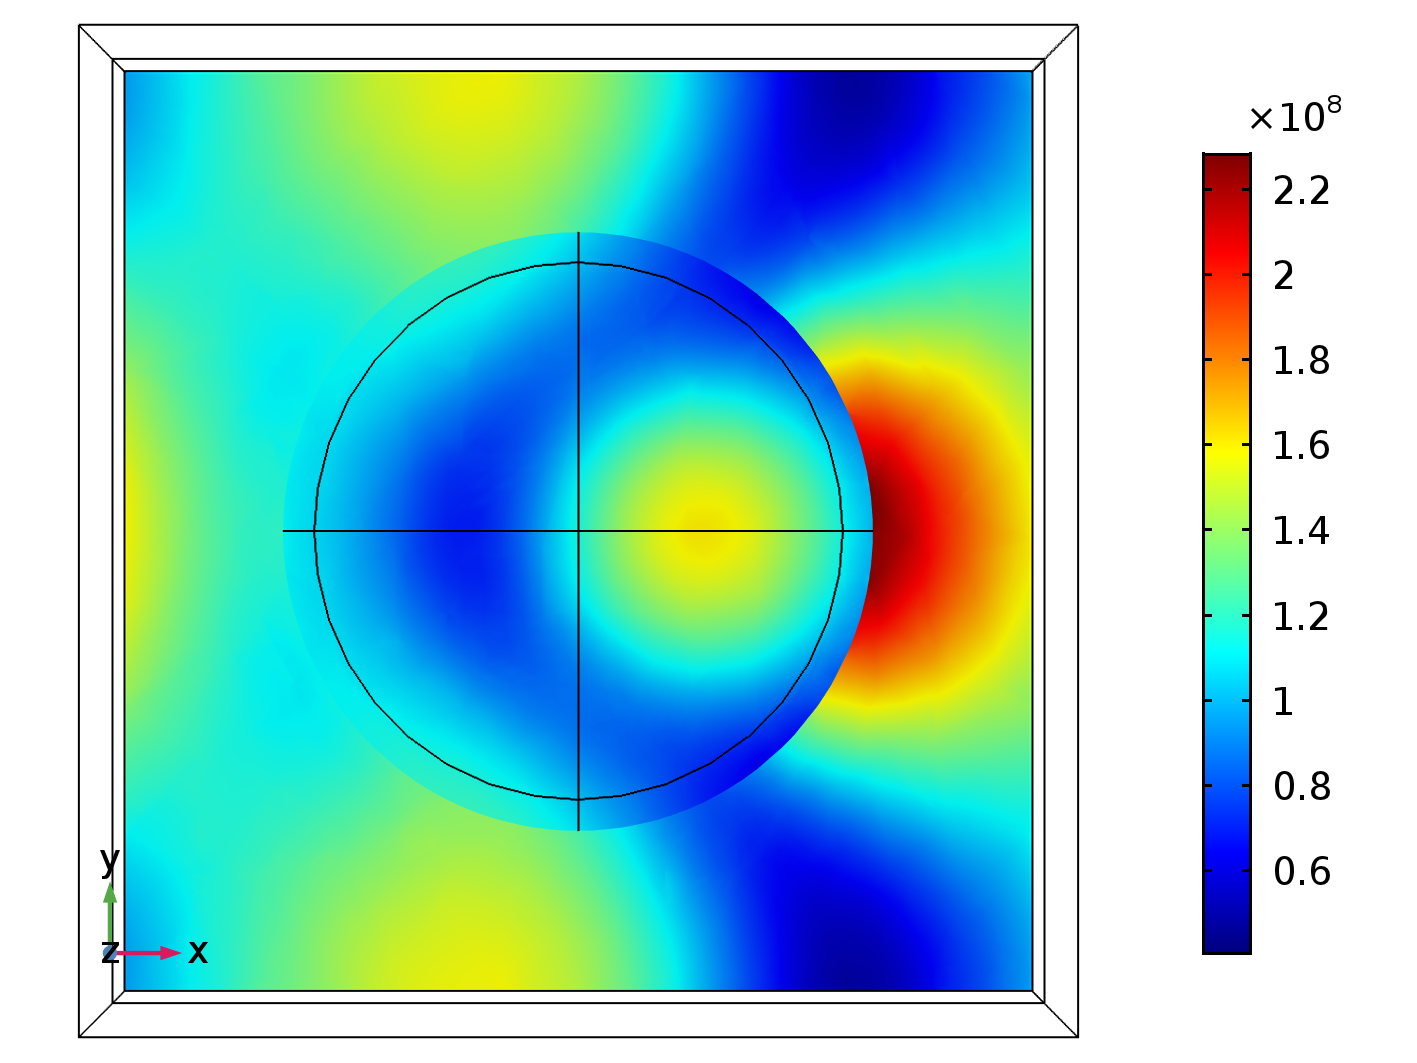
\includegraphics[width=\linewidth]{figures/ch4/S5A/FieldDistribution/Sample5A_TM_Slice@z=-05t_wl=210_notitle.png}
        %\caption{}
   \end{subfigure}
      \begin{subfigure}{0.32\textwidth}
        \centering
        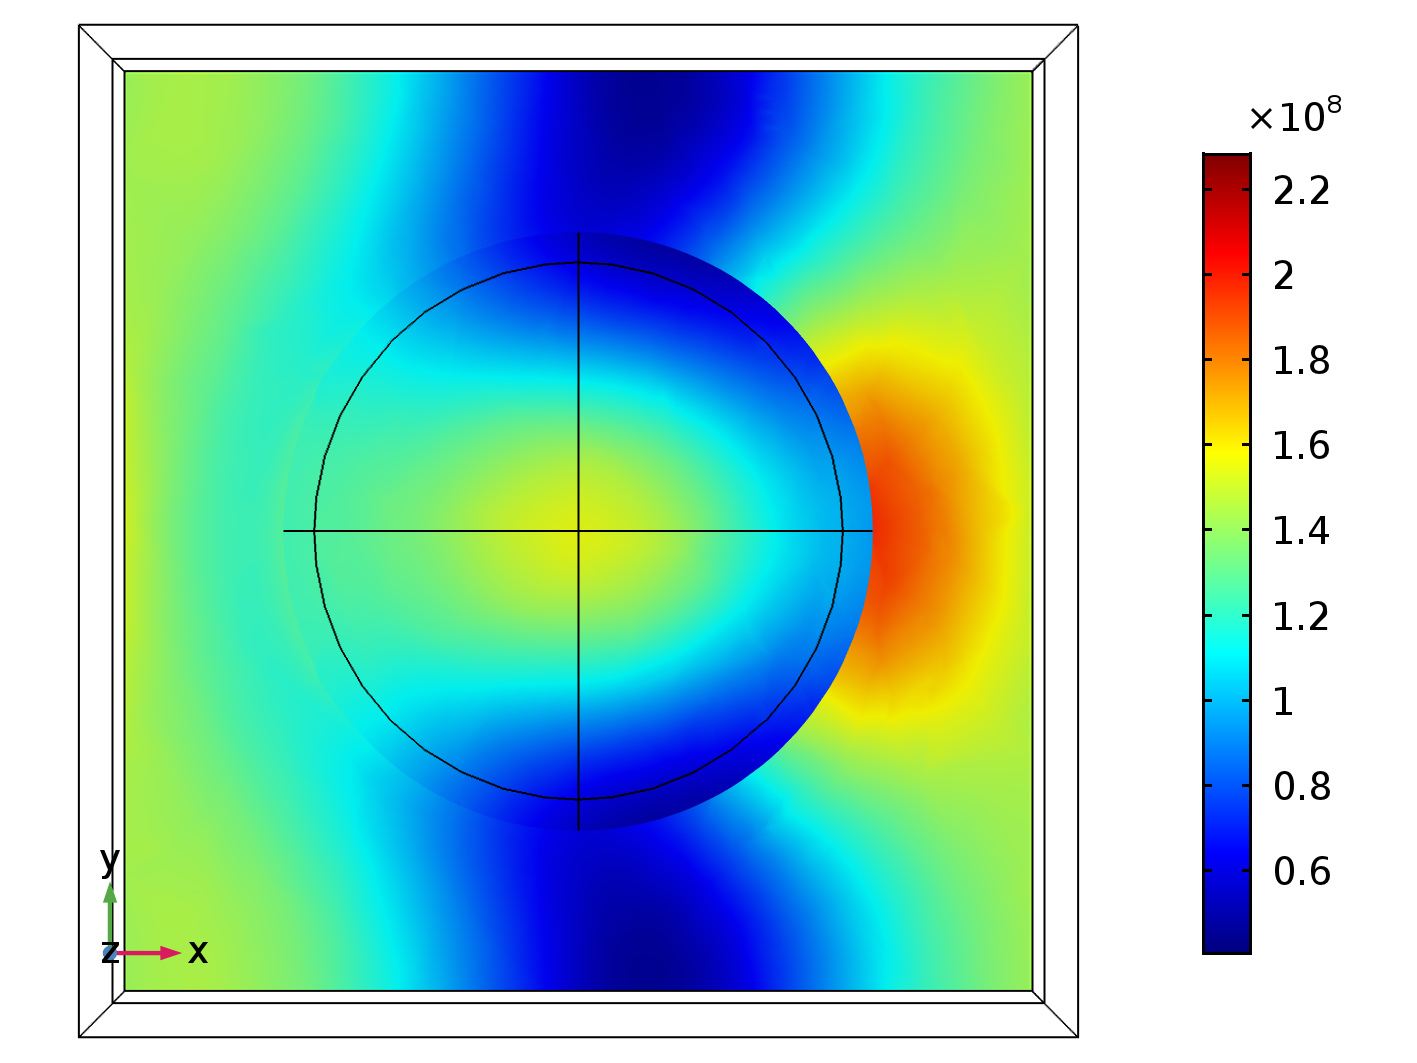
\includegraphics[width=\linewidth]{figures/ch4/S5A/FieldDistribution/Sample5A_TM_Slice@z=-05t_wl=270_notitle.png}
        %\caption{}
   \end{subfigure}
    \begin{subfigure}{0.32\textwidth}
        \centering
        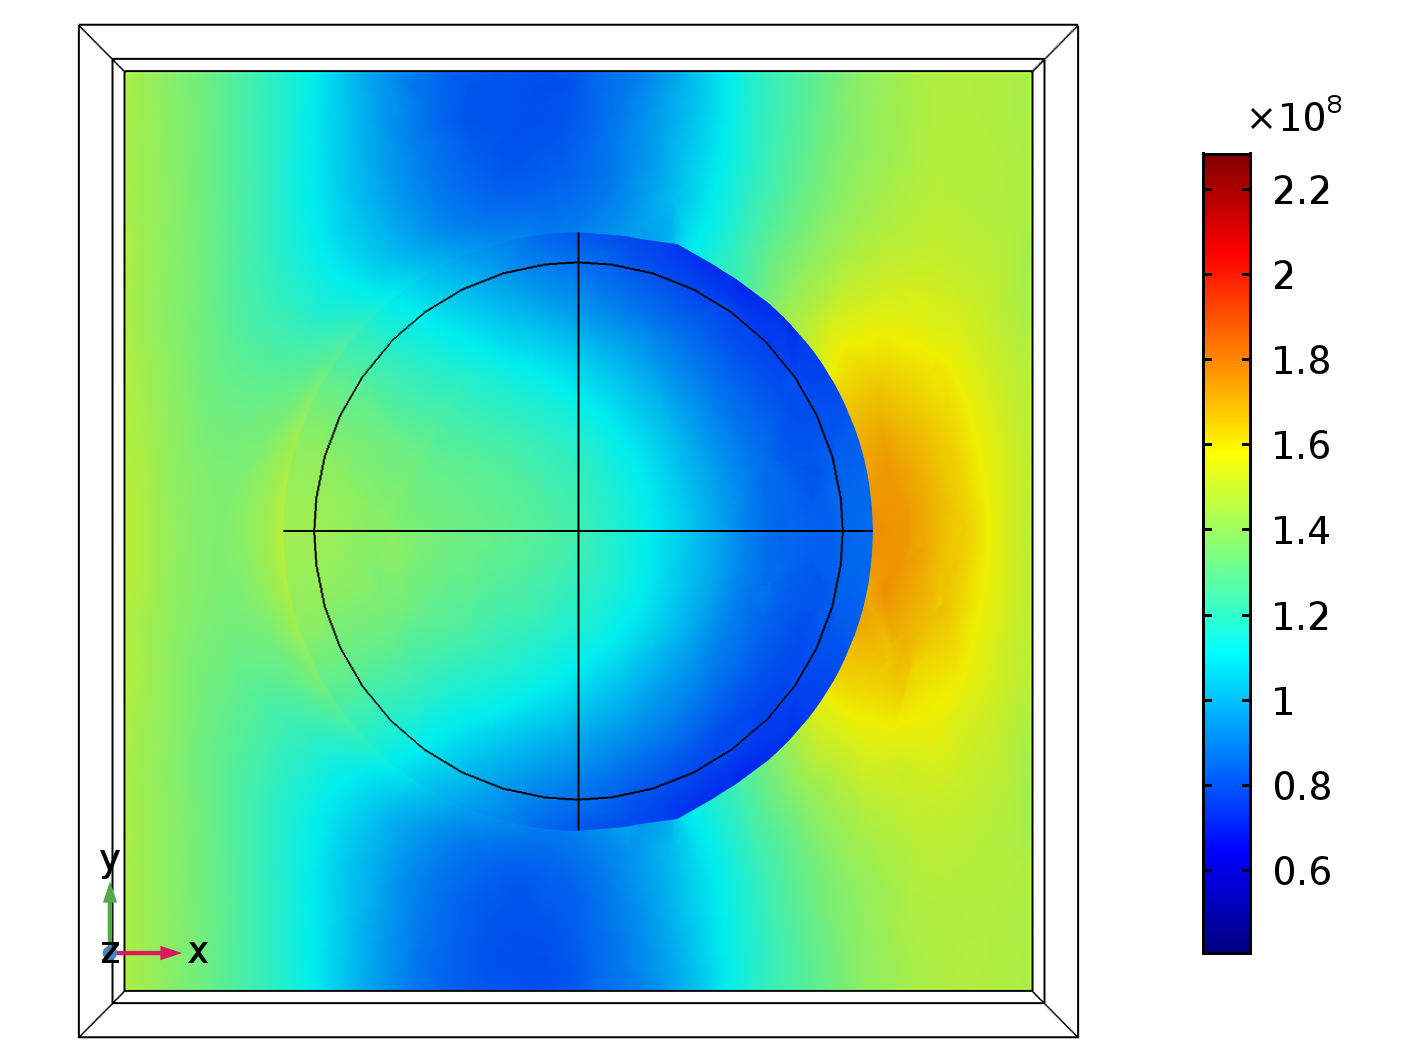
\includegraphics[width=\linewidth]{figures/ch4/S5A/FieldDistribution/Sample5A_TM_Slice@z=-05t_wl=330_notitle.png}
        %\caption{}
   \end{subfigure}
   
   
    \begin{subfigure}{0.32\textwidth}
        \centering
        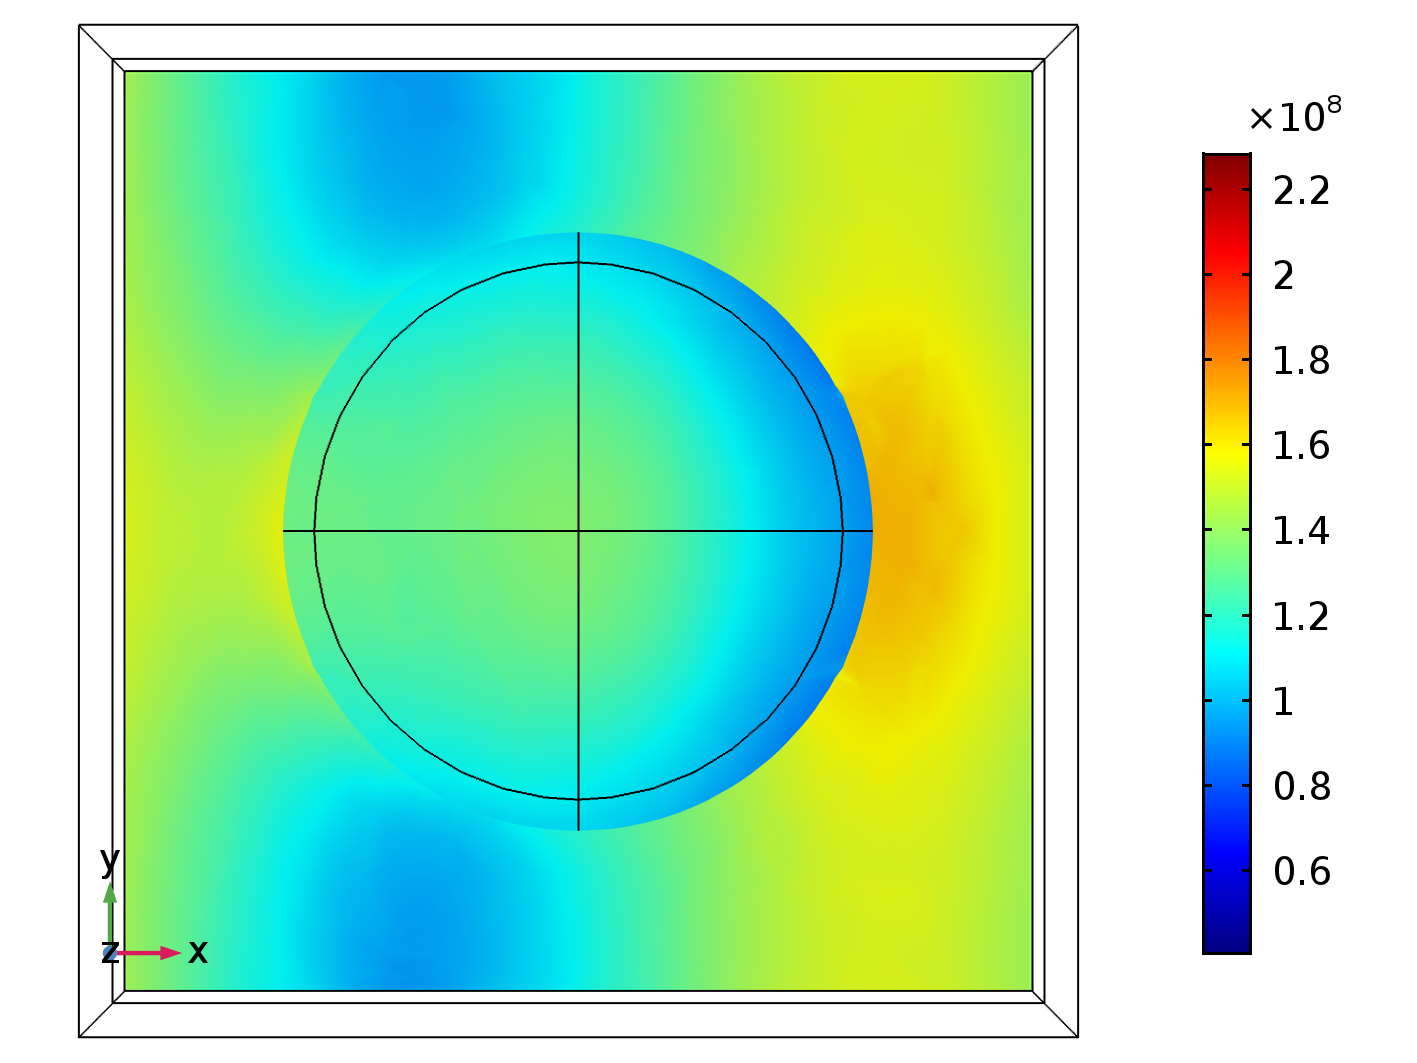
\includegraphics[width=\linewidth]{figures/ch4/S5A/FieldDistribution/Sample5A_TM_Slice@z=-05t_wl=390_notitle.png}
        %\caption{}
        %\vspace{-1cm}
   \end{subfigure}
   \begin{subfigure}{0.32\textwidth}
        \centering
        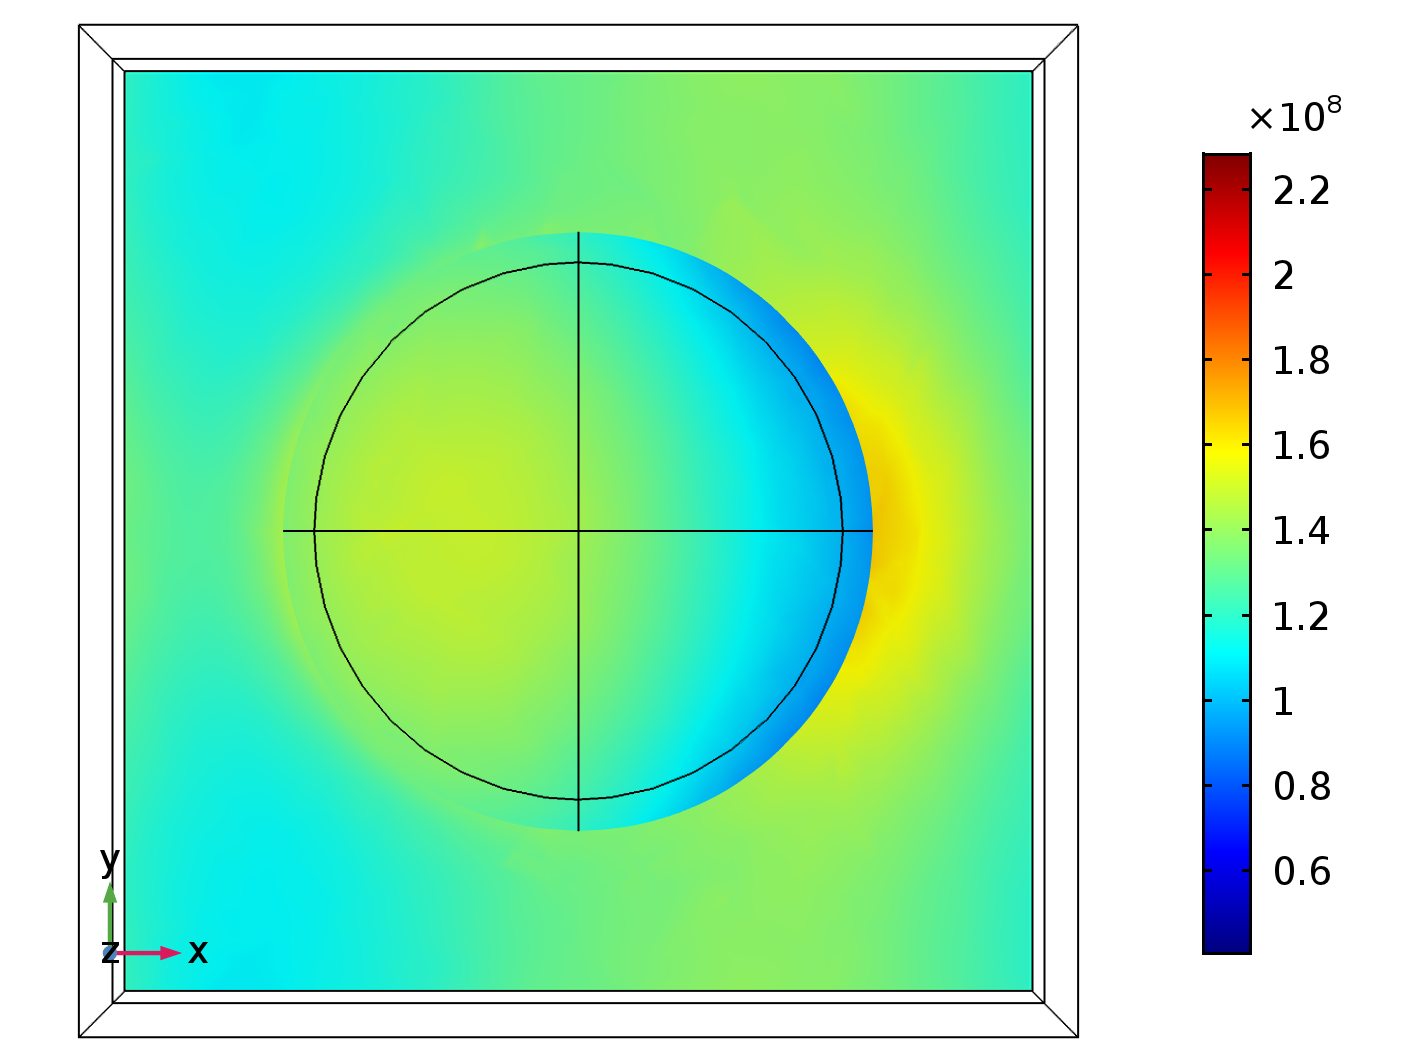
\includegraphics[width=\linewidth]{figures/ch4/S5A/FieldDistribution/Sample5A_TM_Slice@z=-05t_wl=450_notitle.png}
        \caption{TM}
        \vspace{-0.7cm}
   \end{subfigure}   
   \begin{subfigure}{0.32\textwidth}
        \centering
        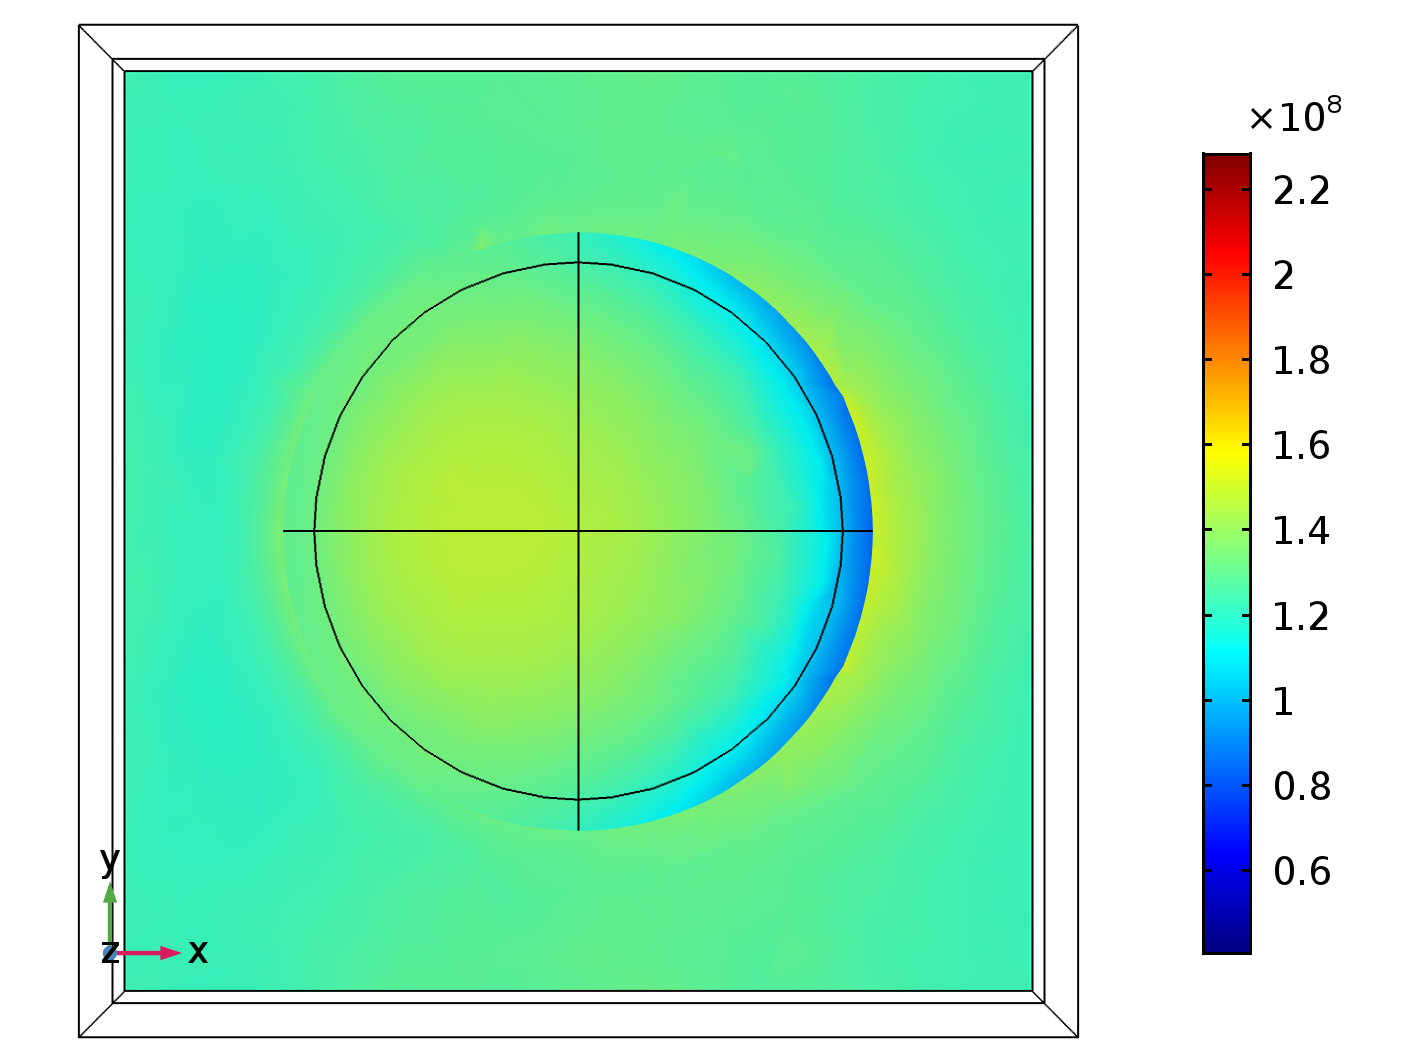
\includegraphics[width=\linewidth]{figures/ch4/S5A/FieldDistribution/Sample5A_TM_Slice@z=-05t_wl=500_notitle.png}
        %\caption{}
        %\vspace{-1cm}
   \end{subfigure}
   \vspace{0.7cm}
   \caption{Electric field norm $E_{\text{norm}}$ at specific wavelengths in the range 210-500 nm, distributed over sample 5A at a cross-section in xy-plane located at $z=-t/2$, as seen from the top of air domain and down towards the gold particle and substrate. The inner black circle marks the edges of the particle at $z=0$, while the outer border-less circle indicate the mound cut right at the middle of its height. (a) shows the electric field norm when the incident light is TE polarized with azimuthal angle $\phi_0=0^\circ$, i.e. beam incident in +x-direction. Similar in (b) for TM-polarization. For both figures, from top left to bottom right, each sub-figure is shown for wavelength $\lambda_0=210 \text{nm}, 270 \text{nm}, 330 \text{nm}, 390 \text{nm}, 450 \text{nm}, 500 \text{nm}$. Axis directions are marked in each sub-figure. The colorbar marks the values for $E_{\text{norm}}$ in units V/m. }
   \label{fig:S5A_normE_distribution_210-500}
\end{figure}

\begin{figure}[htb!]  
    \begin{subfigure}{0.32\textwidth}    %% TE
        \centering
        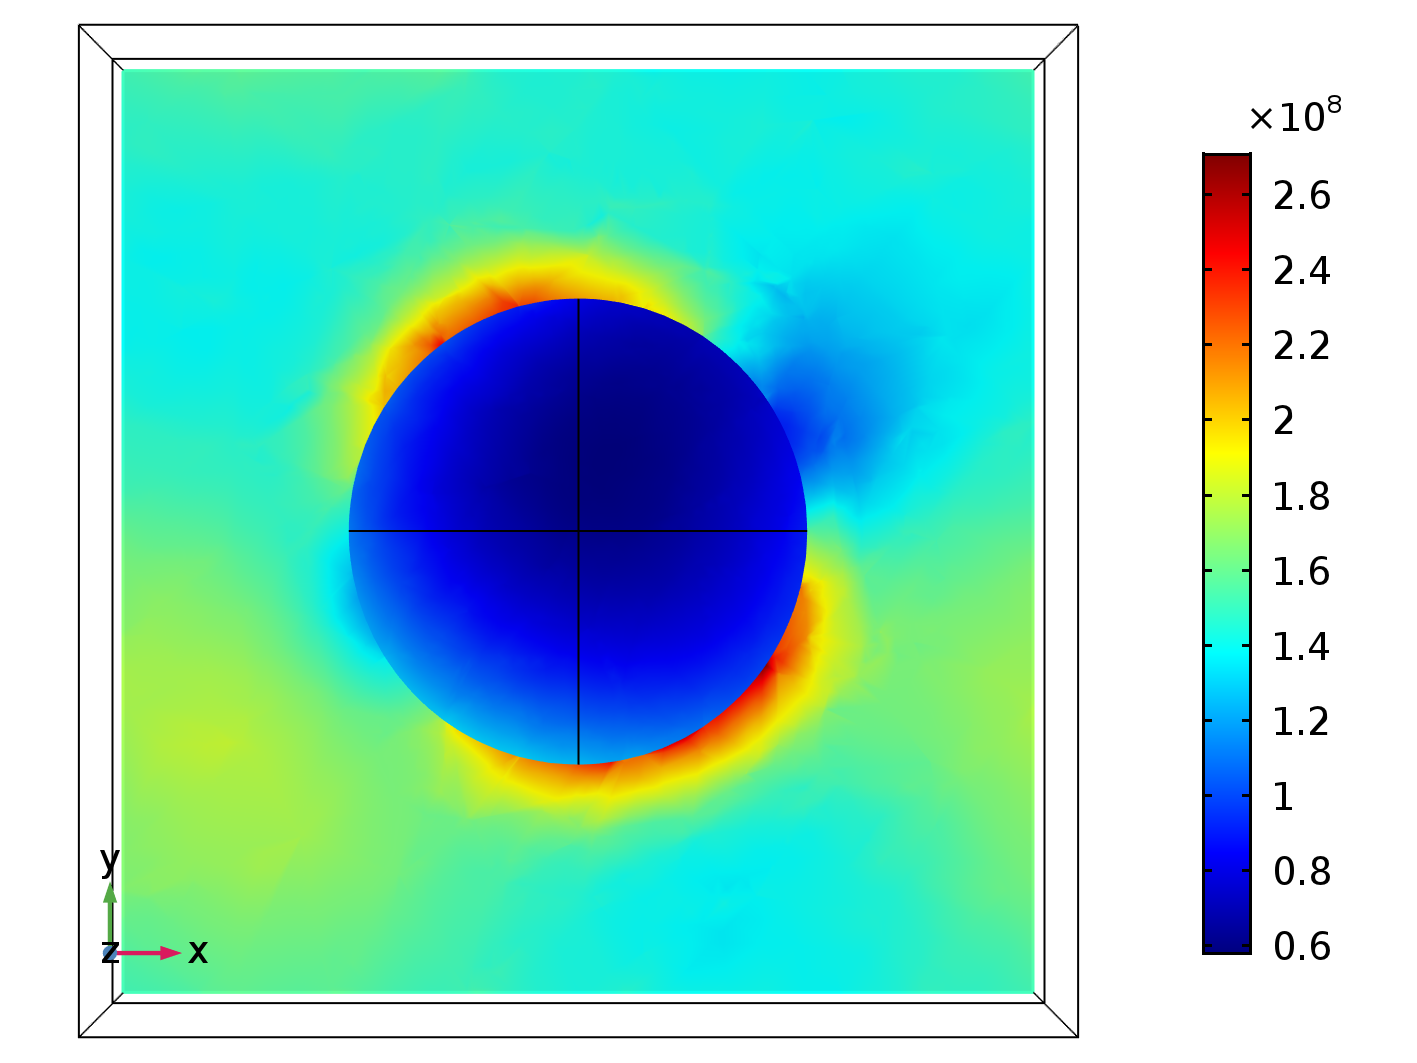
\includegraphics[width=\linewidth]{figures/ch4/S5A/FieldDistribution/phi25/z2/Sample5A_TE_Slice@z=+05Rz_wl=230_phi=25.png}
        %\caption{}
   \end{subfigure}
   \begin{subfigure}{0.32\textwidth}
        \centering
        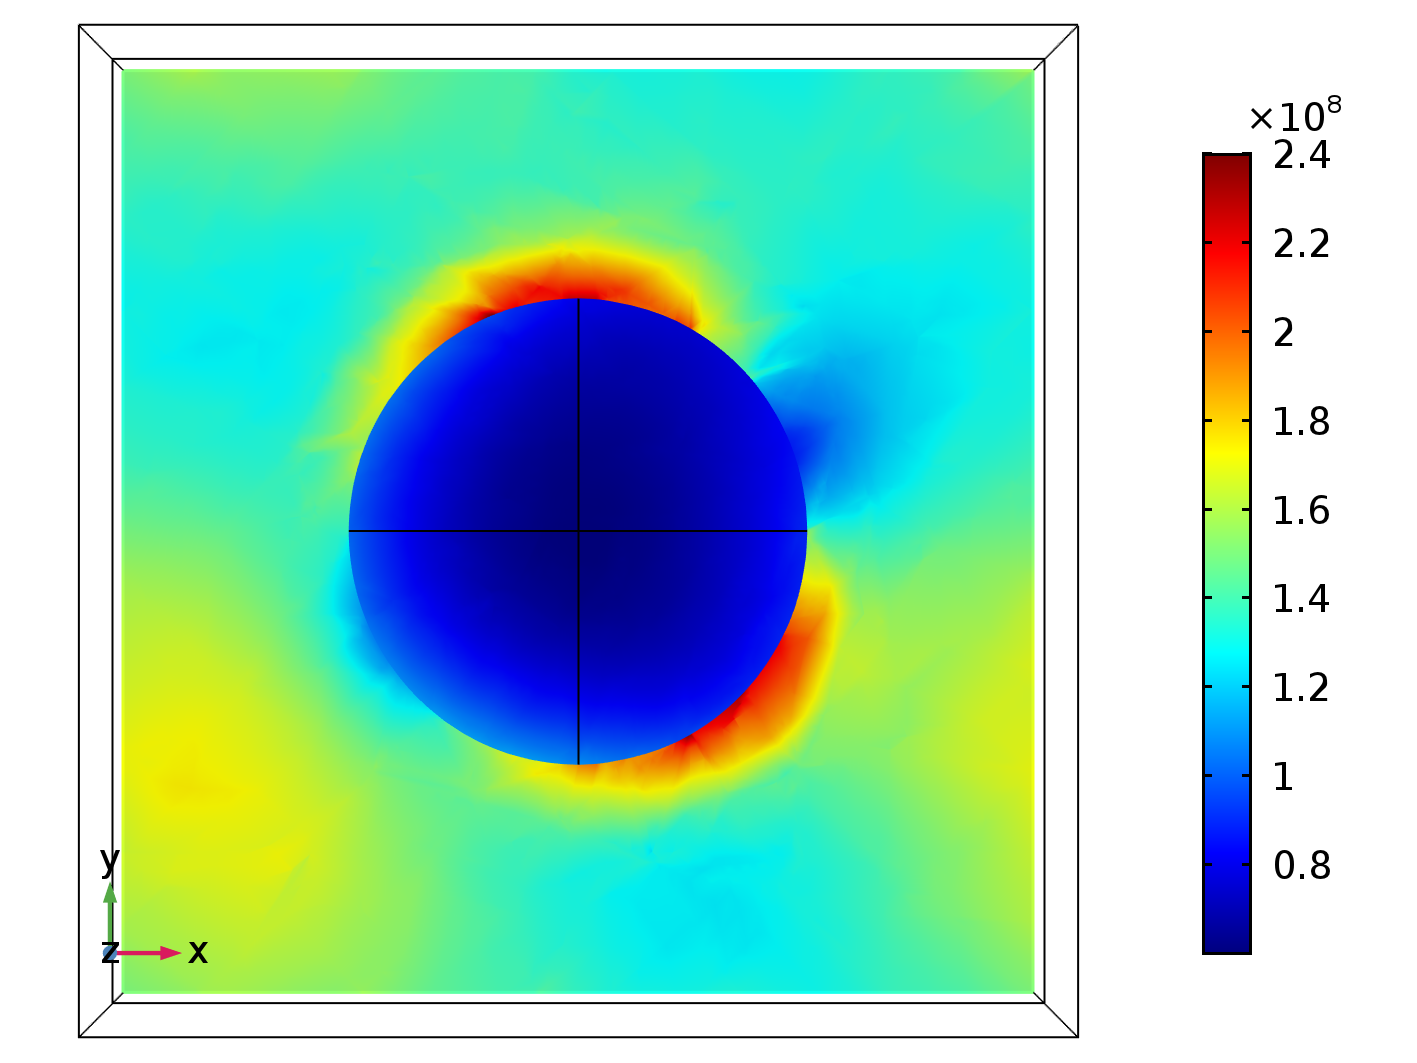
\includegraphics[width=\linewidth]{figures/ch4/S5A/FieldDistribution/phi25/z2/Sample5A_TE_Slice@z=+05Rz_wl=255_phi=25.png}
        %\caption{}
   \end{subfigure}
   \begin{subfigure}{0.32\textwidth}
        \centering
        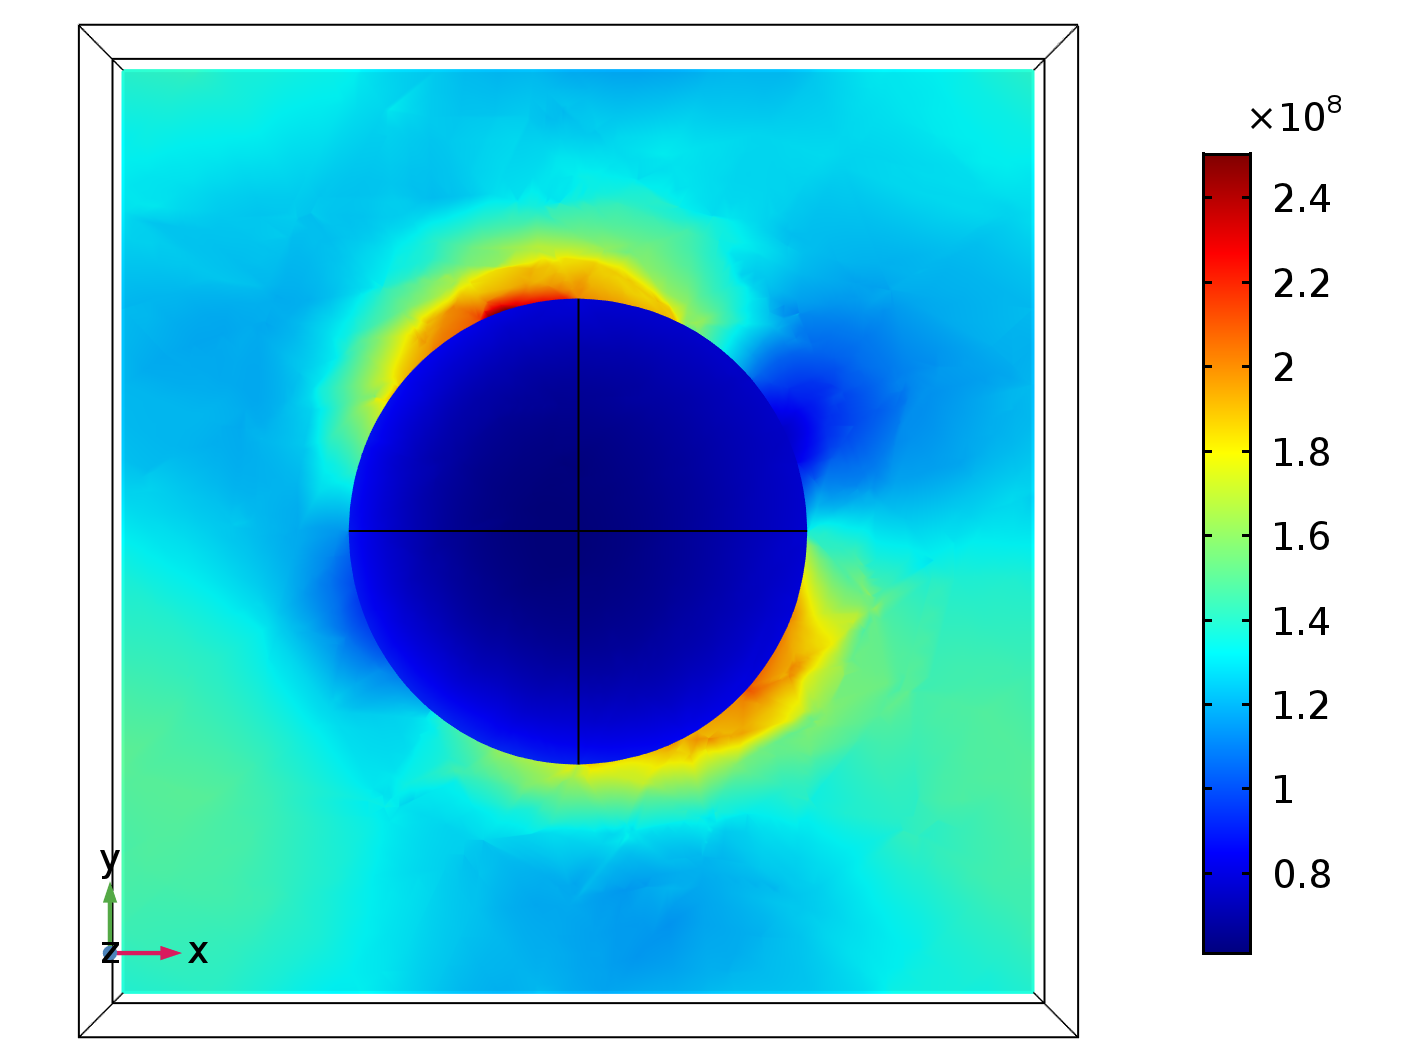
\includegraphics[width=\linewidth]{figures/ch4/S5A/FieldDistribution/phi25/z2/Sample5A_TE_Slice@z=+05Rz_wl=300_phi=25.png}
        %\caption{}
   \end{subfigure}

    \begin{subfigure}{0.32\textwidth}
        \centering
        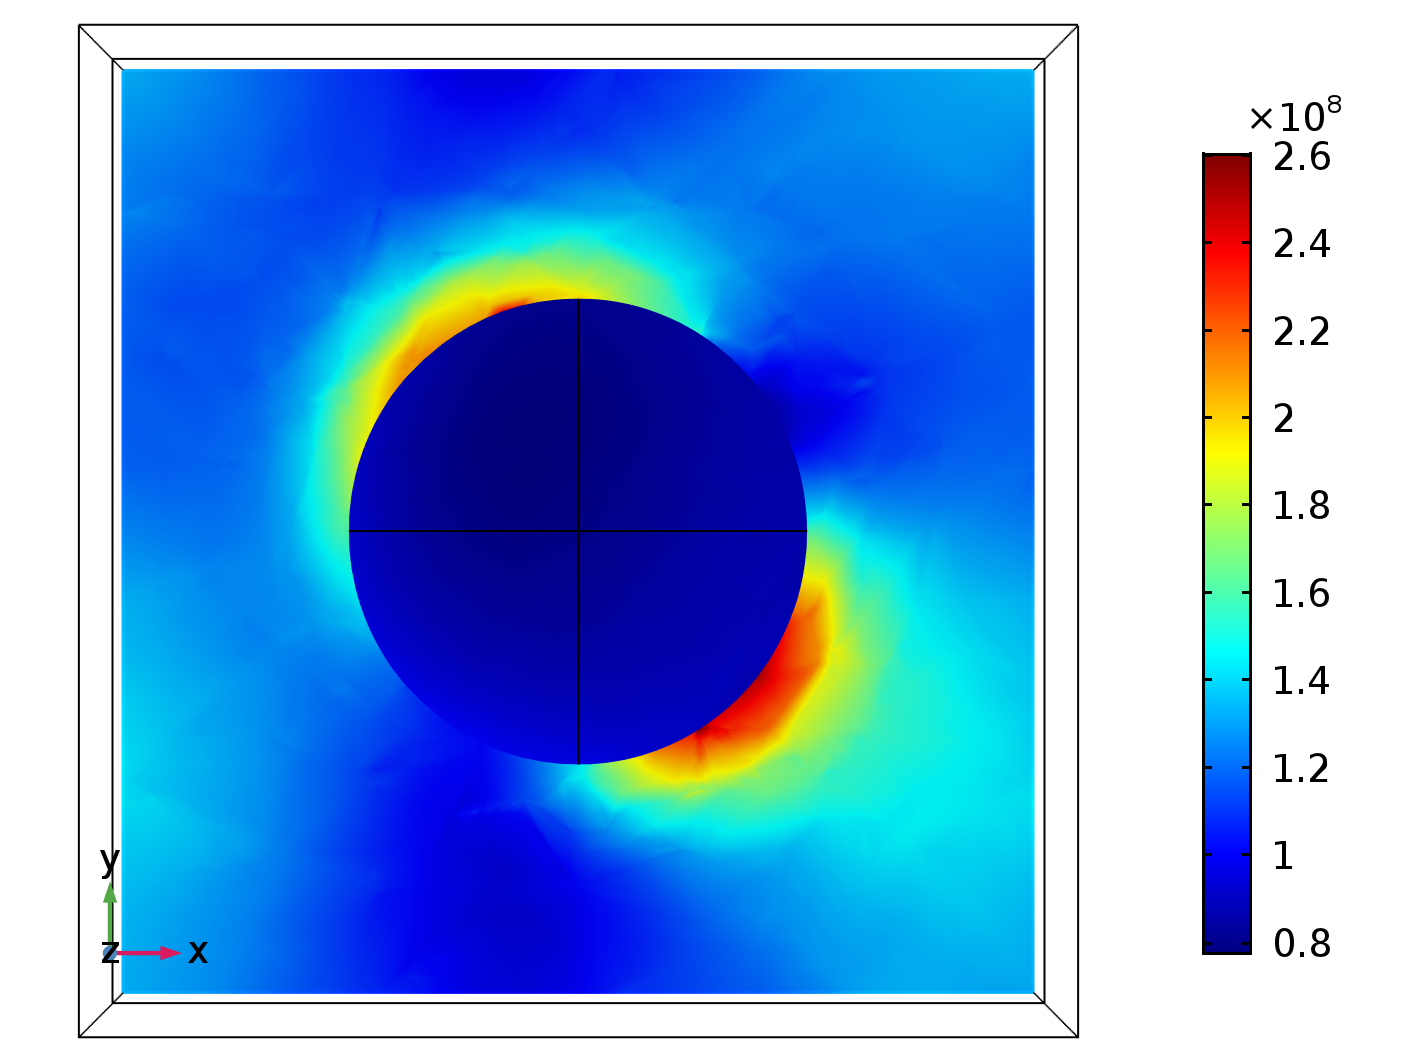
\includegraphics[width=\linewidth]{figures/ch4/S5A/FieldDistribution/phi25/z2/Sample5A_TE_Slice@z=+05Rz_wl=350_phi=25.png}
        %\caption{}
   \end{subfigure}
   \begin{subfigure}{0.32\textwidth}
        \centering
        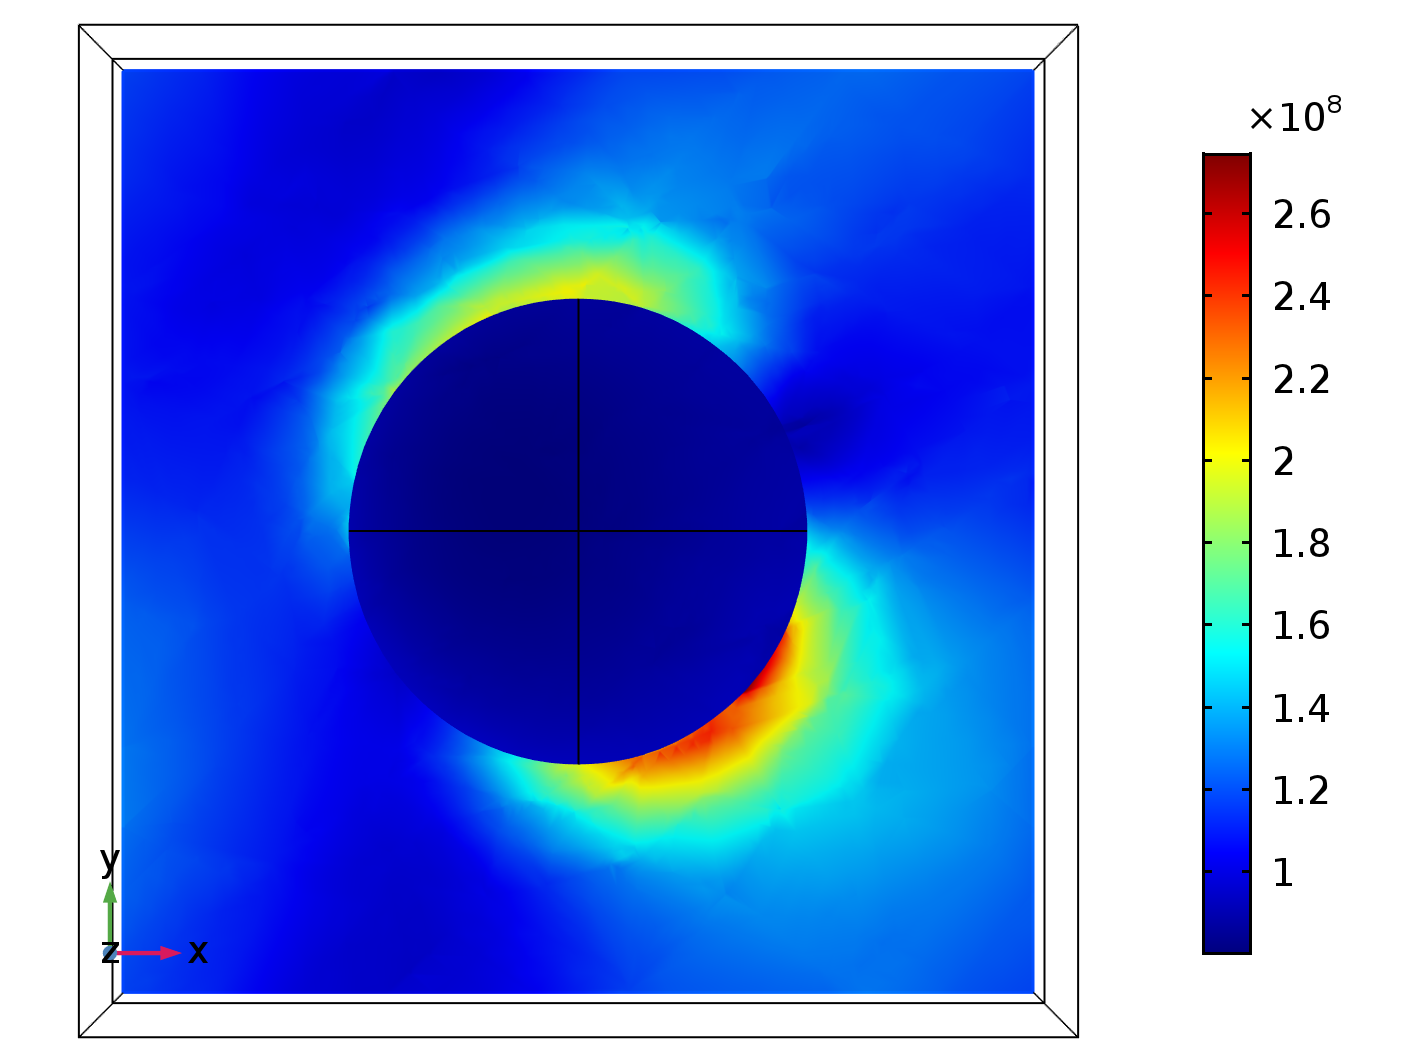
\includegraphics[width=\linewidth]{figures/ch4/S5A/FieldDistribution/phi25/z2/Sample5A_TE_Slice@z=+05Rz_wl=400_phi=25.png}
        \caption{TE}
        \vspace{-0.7cm}
   \end{subfigure}
   \begin{subfigure}{0.32\textwidth}
        \centering
        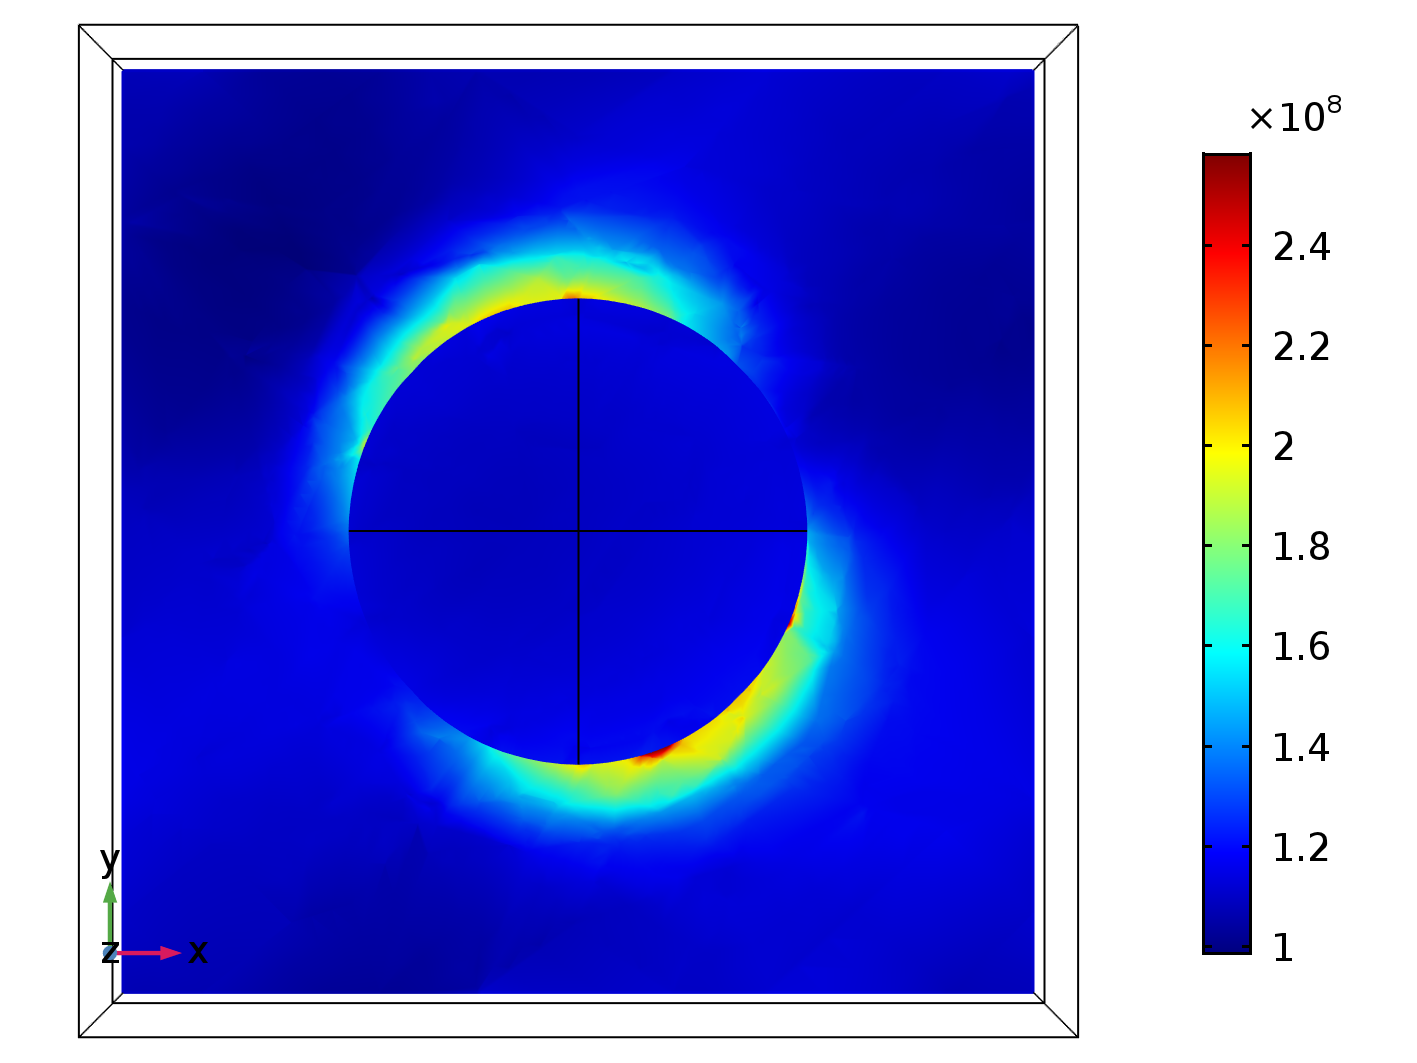
\includegraphics[width=\linewidth]{figures/ch4/S5A/FieldDistribution/phi25/z2/Sample5A_TE_Slice@z=+05Rz_wl=500_phi=25.png}
        %\caption{}
   \end{subfigure}
   \vspace{0.7cm}
   
    \begin{subfigure}{0.32\textwidth}    %% TM
        \centering
        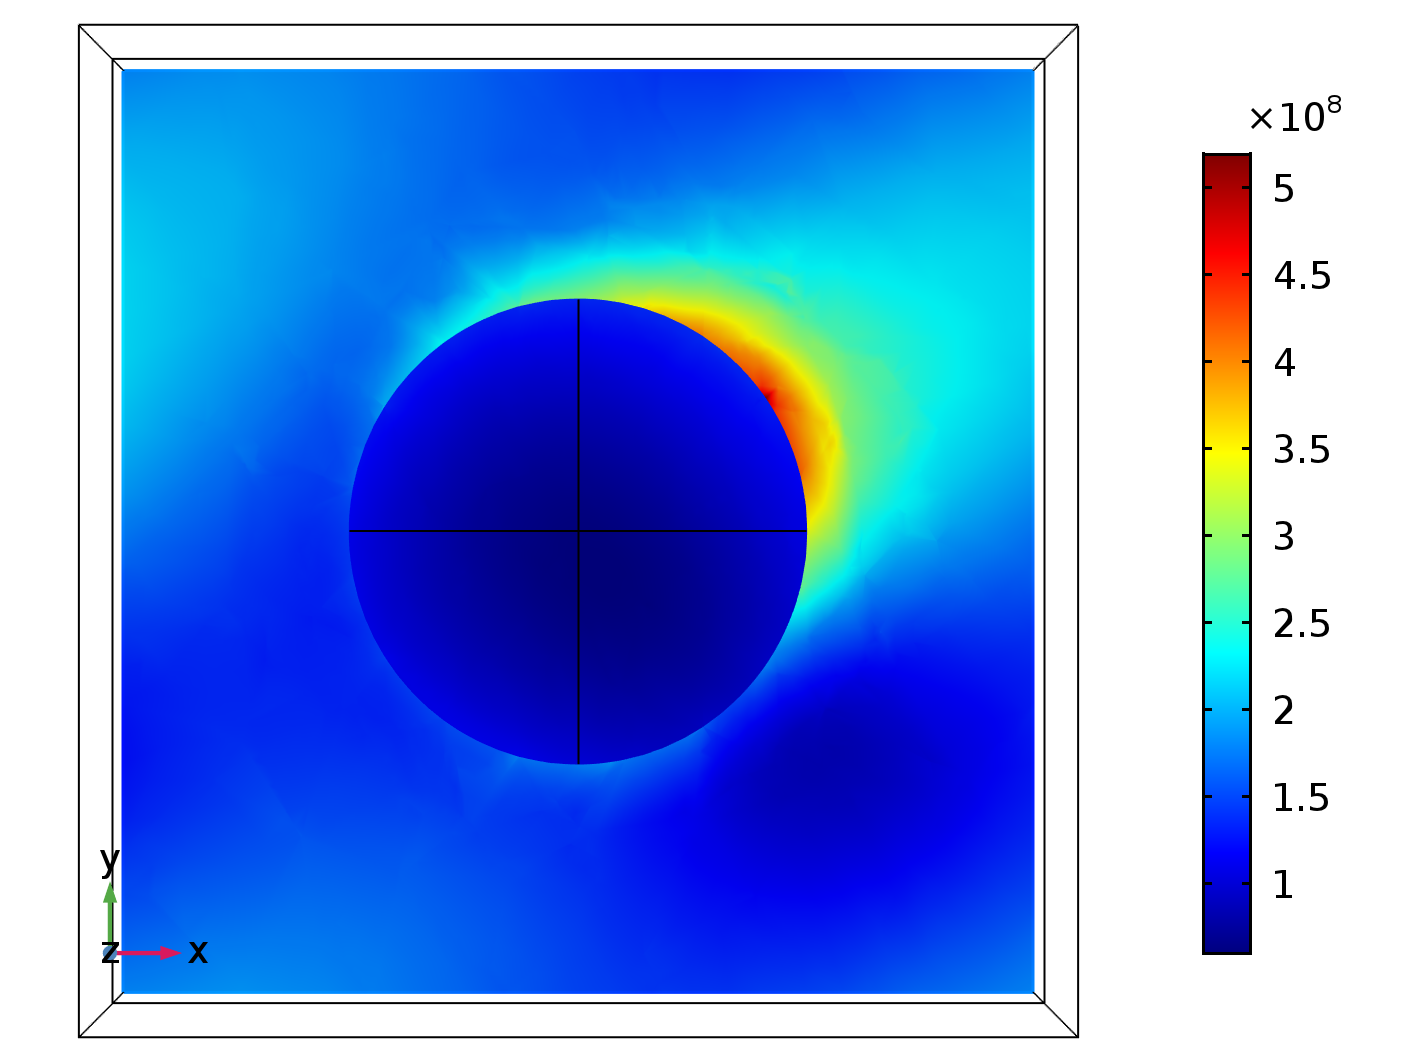
\includegraphics[width=\linewidth]{figures/ch4/S5A/FieldDistribution/phi25/z2/Sample5A_TM_Slice@z=+05Rz_wl=230_phi=25.png}
        %\caption{}
   \end{subfigure}
   \begin{subfigure}{0.32\textwidth}
        \centering
        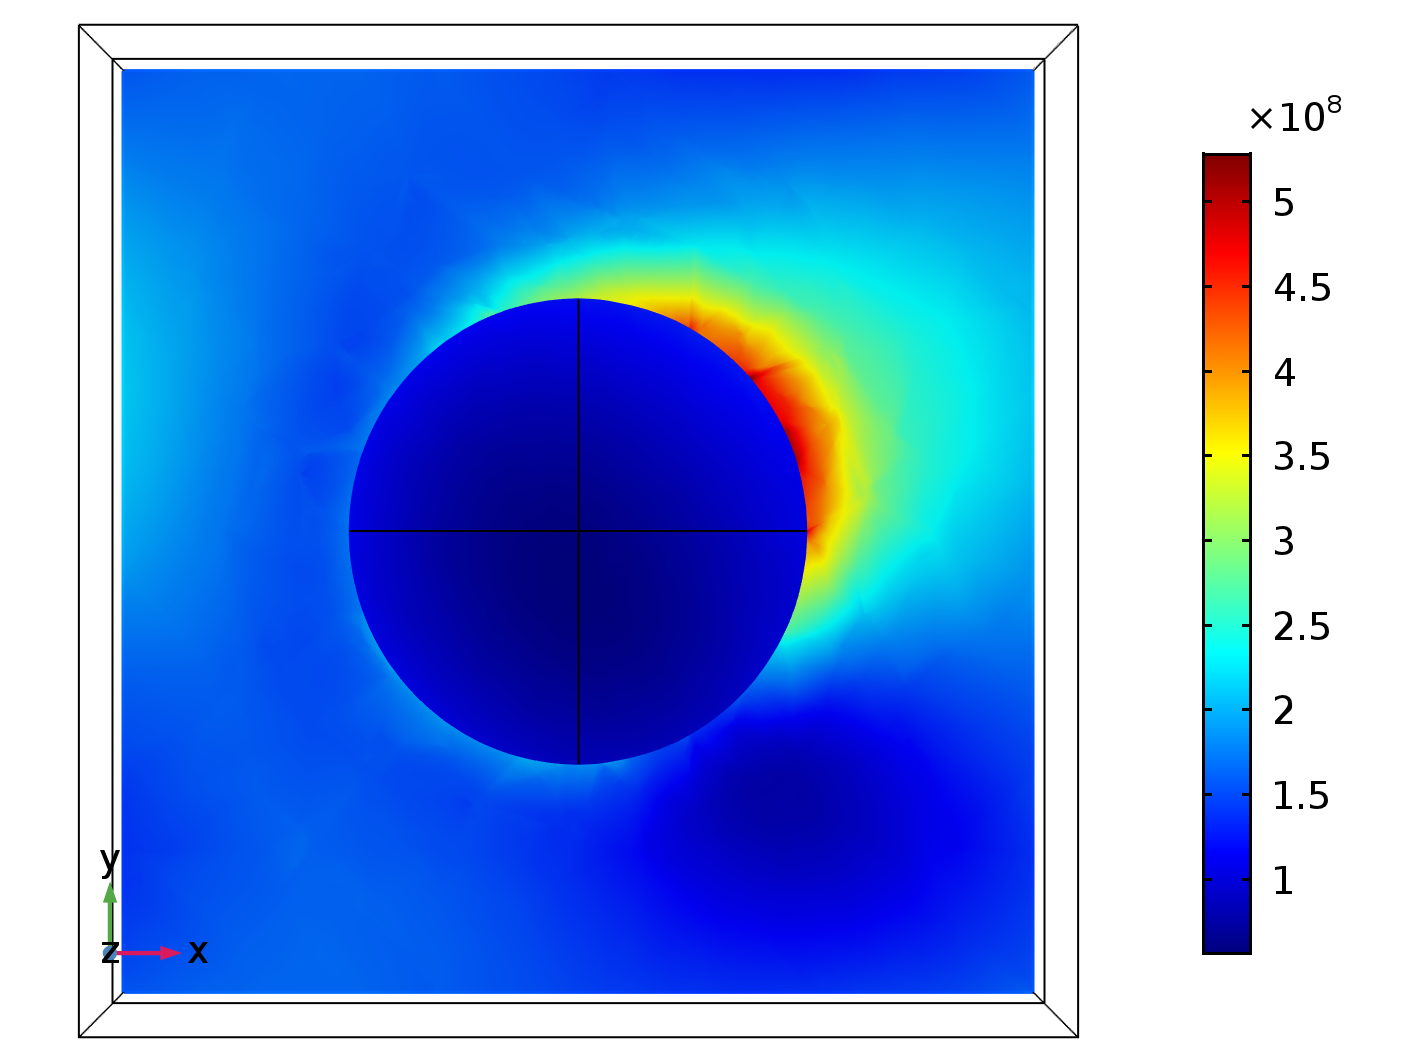
\includegraphics[width=\linewidth]{figures/ch4/S5A/FieldDistribution/phi25/z2/Sample5A_TM_Slice@z=+05Rz_wl=255_phi=25.png}
        %\caption{}
   \end{subfigure}
   \begin{subfigure}{0.32\textwidth}
        \centering
        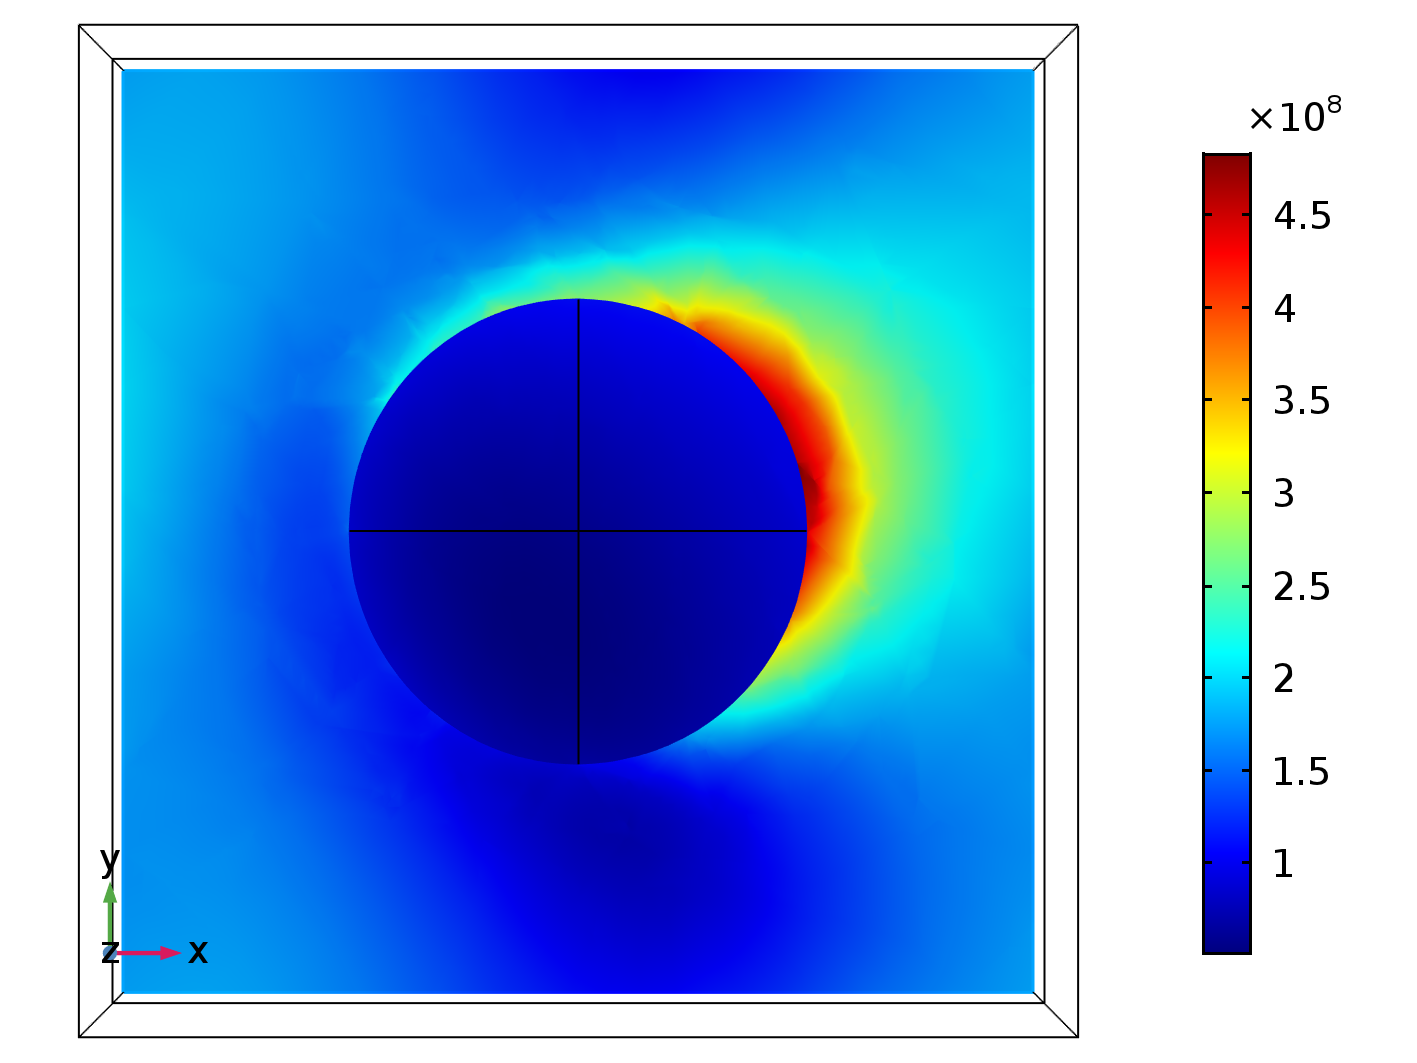
\includegraphics[width=\linewidth]{figures/ch4/S5A/FieldDistribution/phi25/z2/Sample5A_TM_Slice@z=+05Rz_wl=300_phi=25.png}
        %\caption{}
   \end{subfigure}

    \begin{subfigure}{0.32\textwidth}
        \centering
        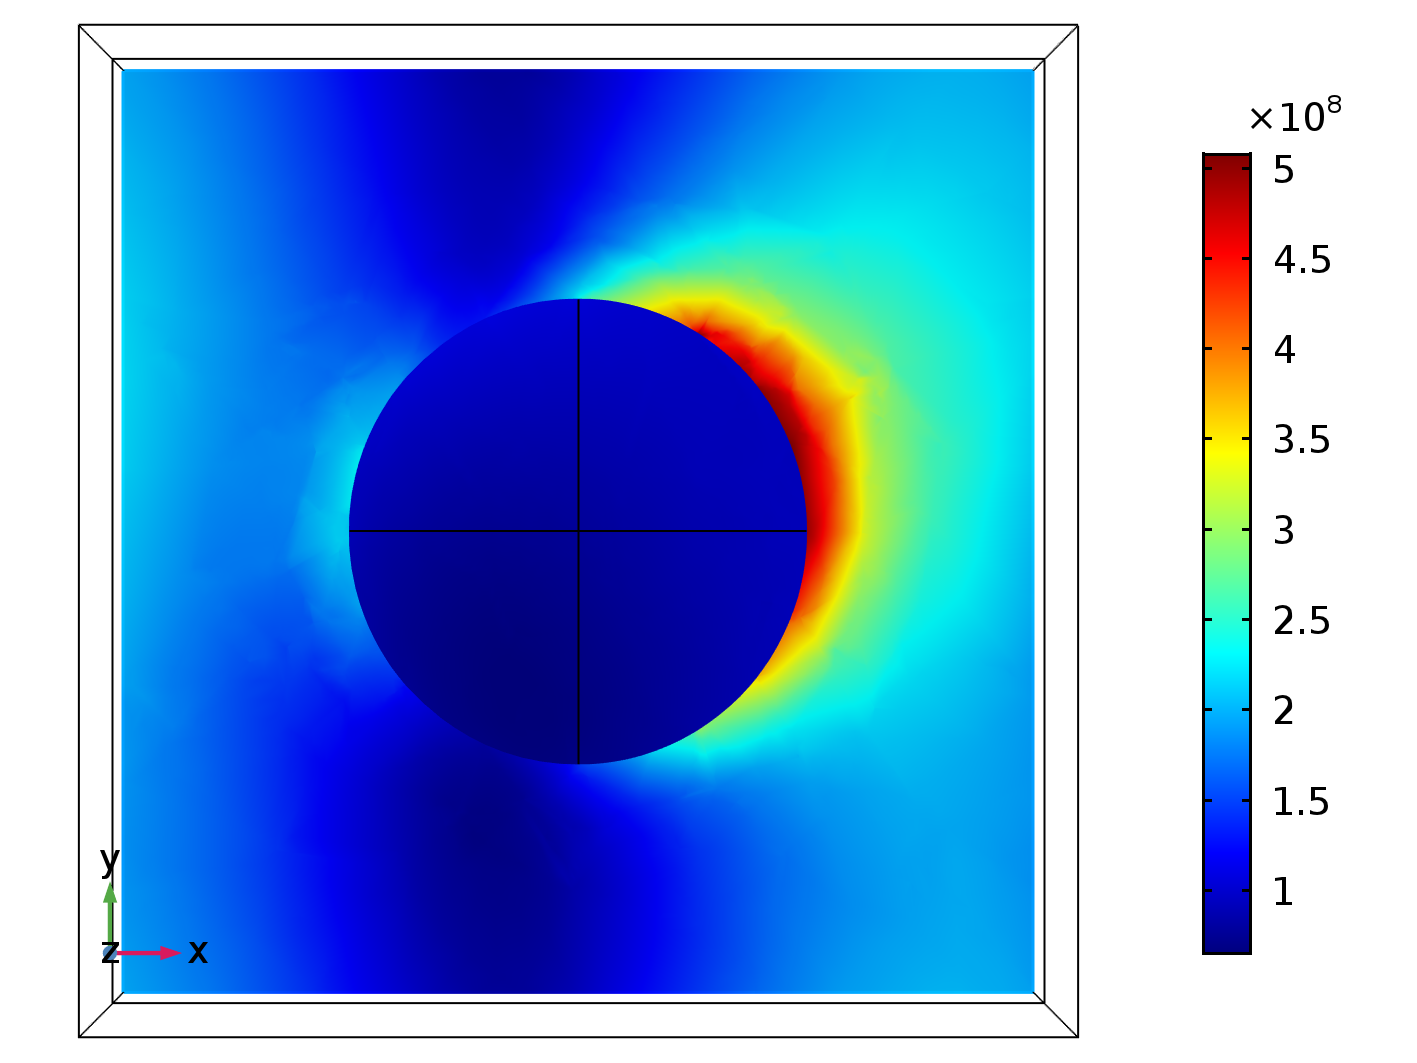
\includegraphics[width=\linewidth]{figures/ch4/S5A/FieldDistribution/phi25/z2/Sample5A_TM_Slice@z=+05Rz_wl=350_phi=25.png}
        %\caption{}
   \end{subfigure}
   \begin{subfigure}{0.32\textwidth}
        \centering
        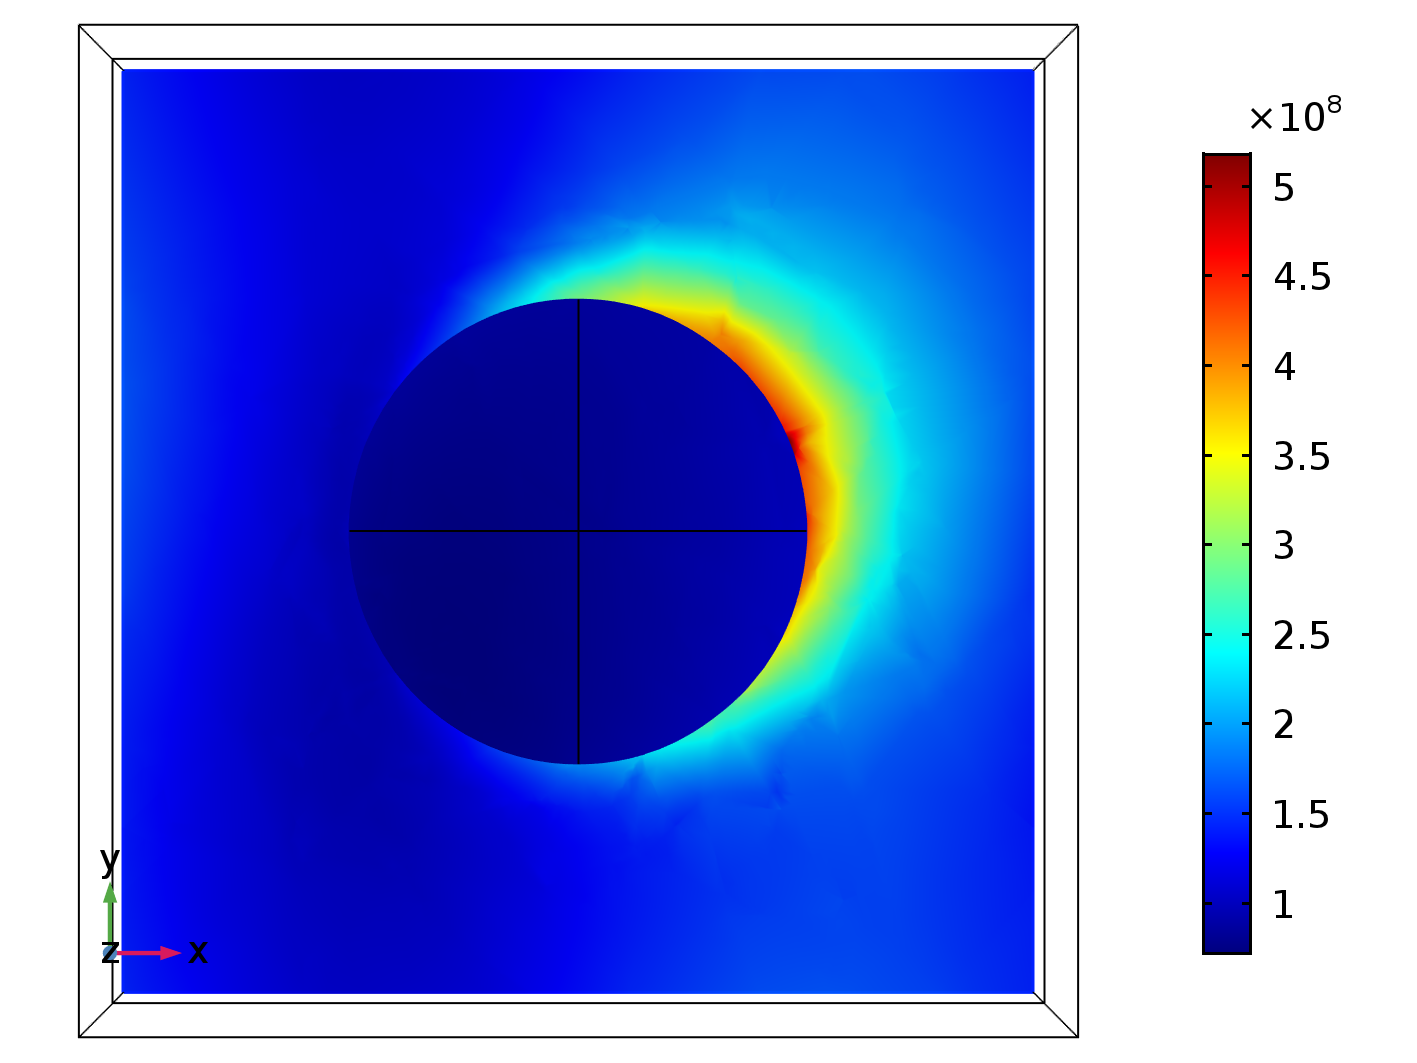
\includegraphics[width=\linewidth]{figures/ch4/S5A/FieldDistribution/phi25/z2/Sample5A_TM_Slice@z=+05Rz_wl=400_phi=25.png}
        \caption{TM}
        \vspace{-0.7cm}
   \end{subfigure}
   \begin{subfigure}{0.32\textwidth}
        \centering
        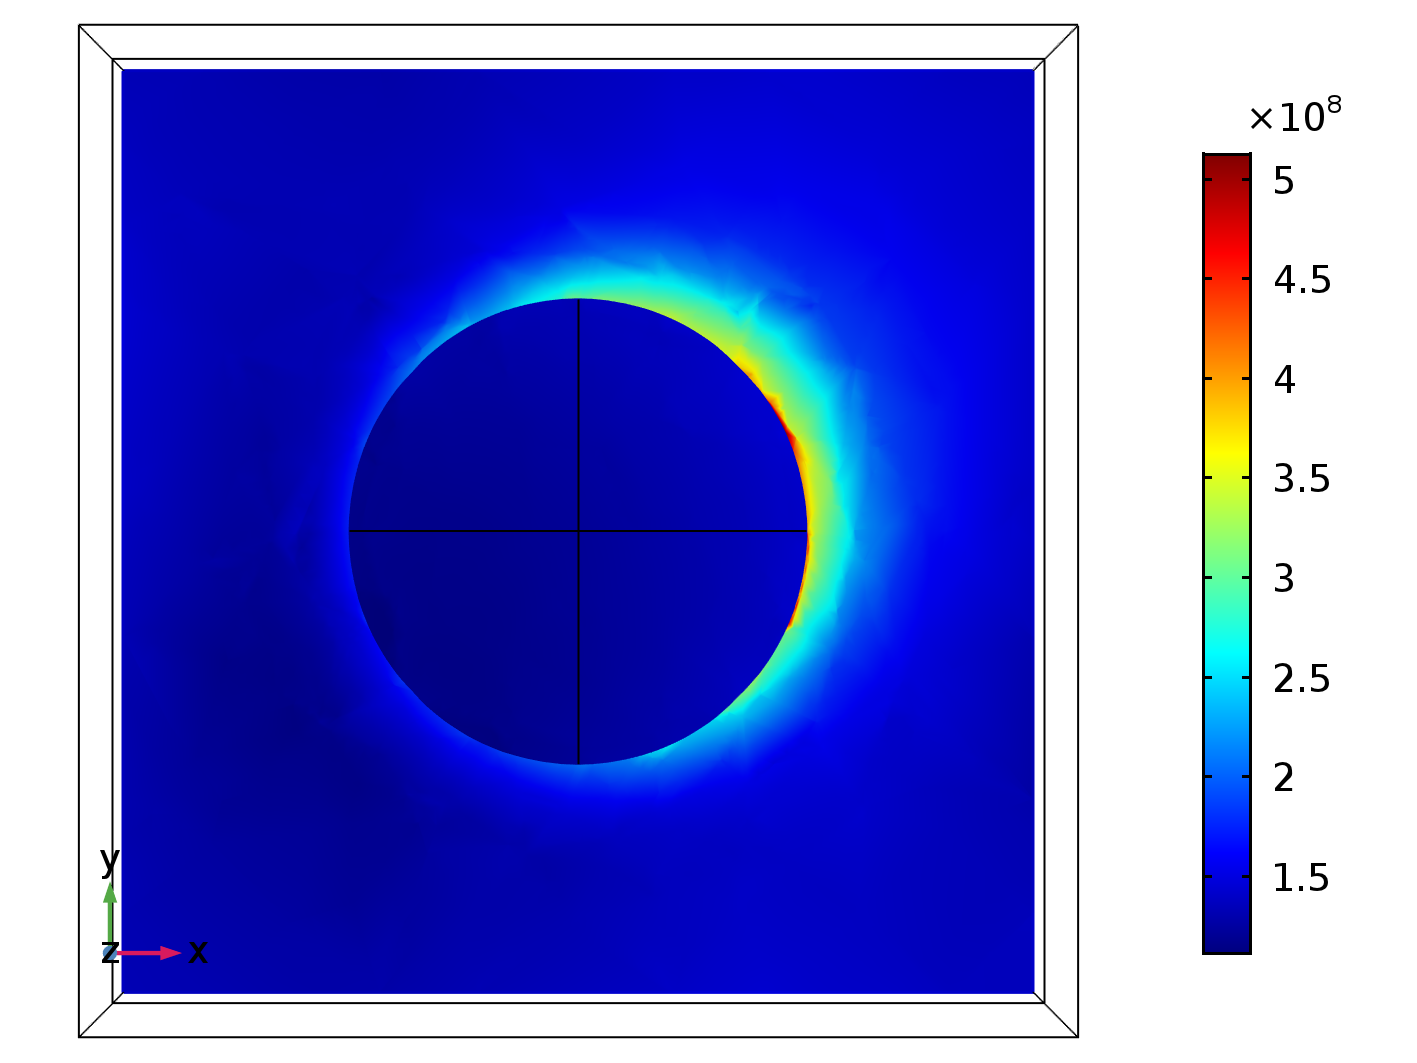
\includegraphics[width=\linewidth]{figures/ch4/S5A/FieldDistribution/phi25/z2/Sample5A_TM_Slice@z=+05Rz_wl=500_phi=25.png}
        %\caption{}
   \end{subfigure}
   \vspace{0.7cm}
   \caption{Identical to figure \ref{fig:S5A_normE_phi25_z=0} only that the cross-section is located at $z=R_z/2$. Azimuthal incident angle $\phi_0=25^\circ$ at wavelengths $\lambda_0=$230nm, 255nm, 300nm, 350nm, 400nm, 500nm, where there is observed polarization coupling.}
   \label{fig:5.10}   
\end{figure}

\chapter{Experimental results}
This appendix presents experimental results of the samples this thesis attempts to recreate numerically. Most figures are plotted anew using the raw data. obtained in CITE [MKpaper, MKpaperBrage, BrakstadMaster, GaSbConespaper]

...


\section{Sample 5A}

\begin{figure}
    \begin{subfigure}{0.5\textwidth}
    \centering
    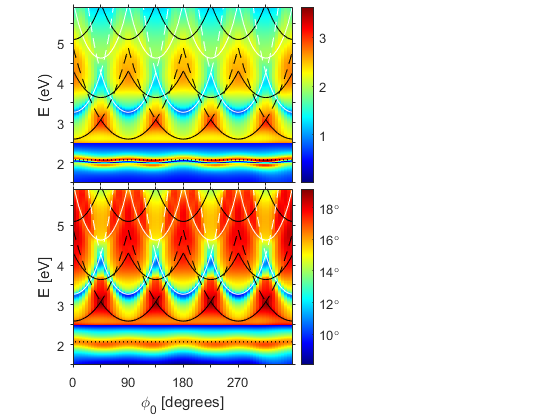
\includegraphics[width=\linewidth, trim=1cm  0cm 5.8cm 0cm, clip]{figures/Appendix/S5A/S5A_eps_psi_all_ExpData.png}
    \caption{$\text{Im}\langle\epsilon_{pp}\rangle$ (top) and $\Psi_{pp}$ (bottom).}
    \label{}
    \end{subfigure}
    \begin{subfigure}{0.5\textwidth}
    \centering
    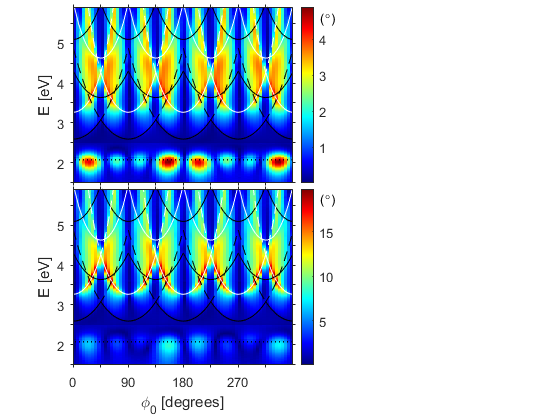
\includegraphics[width=\linewidth, trim=1cm  0cm 5.8cm 0cm, clip]{figures/Appendix/S5A/S5A_psi_sp_ps_all_ExpData.png}
    \caption{$\Psi_{sp}$ (top) and $\Psi_{ps}$ (bottom).}
    \label{}
    \end{subfigure}
    \label{fig:Appendix_S5A_contourplots}
    \caption{Contour plots with azimuthal angle $\phi_0$ and photon energy $E$ of (a) imaginary part of pseudo-dielectric function $\text{Im}\langle\epsilon_{pp}\rangle$ and ellipsometric angle $\Psi_{pp}$, and (b) ellipsometric angles $\Psi_{ps}$ and $\Psi_{sp}$, for experimental values of sample 5A. Horizontal dotted line highlights the energy position of the LSPR around 2.08 eV. Rayleigh lines corresponding to boundaries of 1st BZ (lower energy) and 2nd BZ (higher energy) are shown as white lines (air) and black lines (substrate). Dashed lines indicate their respective extended Rayleigh lines. A scaling has been applied for values where photonic energy is $E<2.5$ eV, so that plotted quantities in this range is (a) $\text{Im}\langle\epsilon_{pp}\rangle$/5.6 and $\Psi_{pp}$/2, (b) 2$\Psi_{ps}$ and 2$\Psi_{sp}$.}
\end{figure}